    %%%%%%%%%%%%%%%%%%%%%%%%%%%%%%%%%%%%%%%%%%%%%%%%%%%%%%%%%%%%
%%  This Beamer template was created by Cameron Bracken.
%%  Anyone can freely use or modify it for any purpose
%%  without attribution.
%%
%%  Last Modified: January 9, 2009
%%

\documentclass[xcolor=x11names,compress]{beamer}

%% General document %%%%%%%%%%%%%%%%%%%%%%%%%%%%%%%%%%
\usepackage{graphicx}
\usepackage{pgfplots}
\usepackage{epstopdf}
\usepackage{tikz}
\usepackage{siunitx}
\usepackage{tikz}
\usetikzlibrary{arrows,automata}
\usepackage{siunitx}
\usepackage{pgf}
\usetikzlibrary{arrows}
\usetikzlibrary{decorations.fractals, arrows}
\usetikzlibrary{arrows,decorations.pathreplacing}
\usepackage{xcolor}
\usetikzlibrary{arrows, shapes, calc}
%%%%%%%%%%%%%%%%%%%%%%%%%%%%%%%%%%%%%%%%%%%%%%%%%%%%%%
\usepackage{qtree} 
\usepackage{epstopdf}
%% Beamer Layout %%%%%%%%%%%%%%%%%%%%%%%%%%%%%%%%%%
\useoutertheme[subsection=false,shadow]{miniframes}
\useinnertheme{default}
\usefonttheme{serif}
\usepackage{palatino}
\setcounter{tocdepth}{1}

\setbeamerfont{title like}{shape=\scshape}
\setbeamerfont{frametitle}{shape=\scshape}

\setbeamercolor*{lower separation line head}{bg=DeepSkyBlue4}
\setbeamercolor*{normal text}{fg=black,bg=white}
\setbeamercolor*{alerted text}{fg=red}
\setbeamercolor*{example text}{fg=black}
\setbeamercolor*{structure}{fg=black}

\setbeamercolor*{palette tertiary}{fg=black,bg=black!10}
\setbeamercolor*{palette quaternary}{fg=black,bg=black!10}

% Page numbering
\addtobeamertemplate{navigation symbols}{}{%
    \usebeamerfont{footline}%
    \usebeamercolor[fg]{footline}%
    \hspace{1em}%
    \insertframenumber/\inserttotalframenumber
}

\renewcommand{\(}{\begin{columns}}
\renewcommand{\)}{\end{columns}}
\newcommand{\<}[1]{\begin{column}{#1}}
\renewcommand{\>}{\end{column}}
\tikzset{onslide/.code args={<#1>#2}{%
  \only<#1>{\pgfkeysalso{#2}} % \pgfkeysalso doesn't change the path
}}  
%%%%%%%%%%%%%%%%%%%%%%%%%%%%%%%%%%%%%%%%%%%%%%%%%%
\beamertemplatenavigationsymbolsempty % remove navigation bar 


\begin{document}


%%%%%%%%%%%%%%%%%%%%%%%%%%%%%%%%%%%%%%%%%%%%%%%%%%%%%%
%%%%%%%%%%%%%%%%%%%%%%%%%%%%%%%%%%%%%%%%%%%%%%%%%%%%%%

%%    INPUT    %%%
\section{\scshape Introduction}
\subsection{Probabilistic Automata}

\begin{frame}
	\begin{center}
		\Large{Learning Probabilistic Automata}
		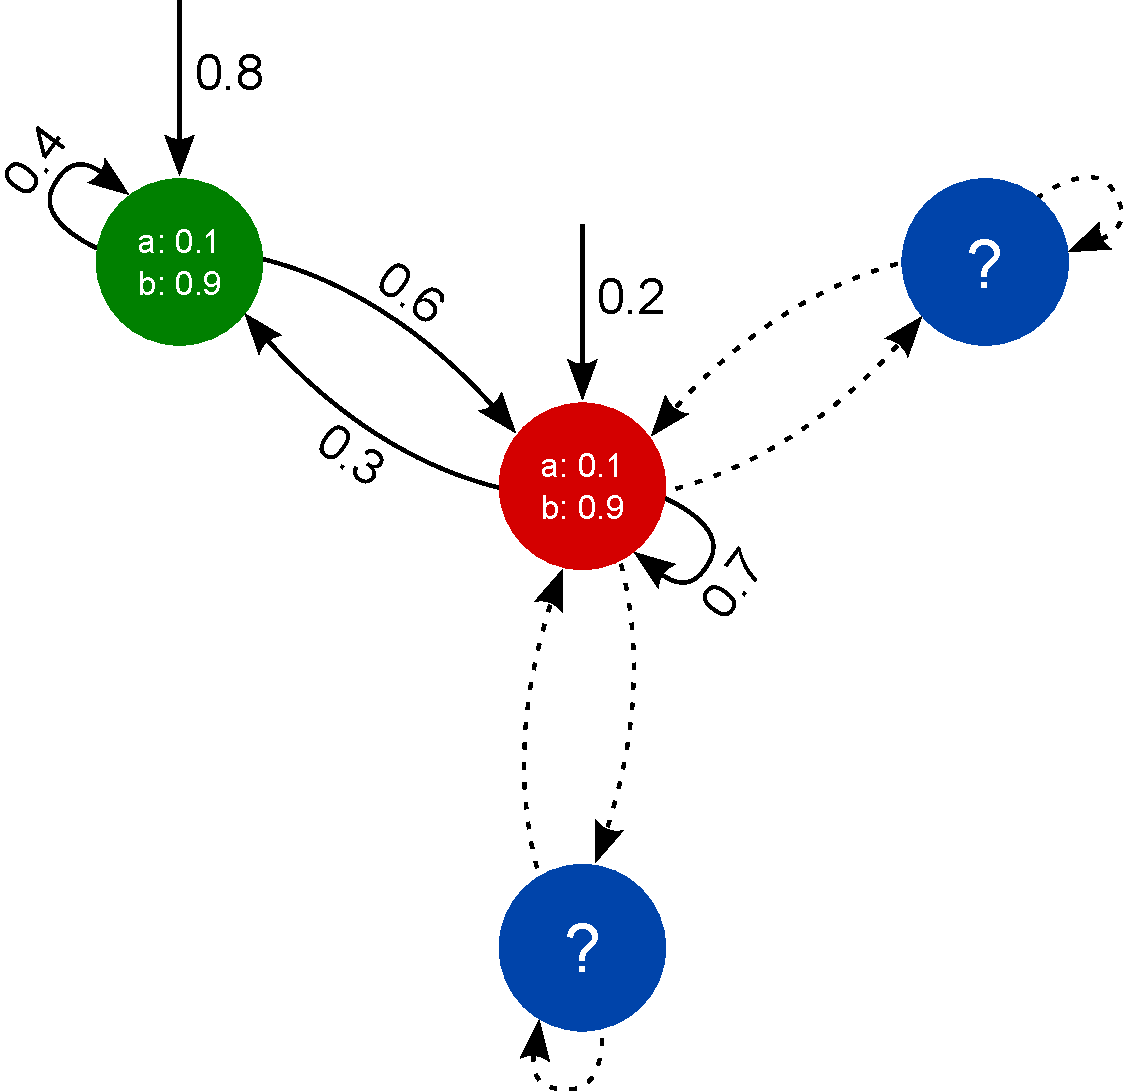
\includegraphics[width=0.48\textwidth]{images/frontpagemodel.pdf}\\
		\small{\textbf{Mathias M. Andersen\\
		Kent M. Caspersen\\
		Anders R. Nielsen\\
		Juraj Kol\v{c}\'{a}k\\
		Guillaume Grippari\\
		Theis Christensen\\}}
	\end{center}
\end{frame}

\begin{frame}
	\begin{center}
		\frametitle{Models}
		
		$$n~grams \parallel Markov~chains < DPFA <$$
		
		$$< HMM \approx PFA <$$
		
		$$< Multiplicity~automata$$
	\end{center}
\end{frame}

\subsection{PAutomaC}

\begin{frame}
	\frametitle{\emph{PAutomaC}}
	\begin{itemize}
		\item 2012 online PFA learning competition.
		\item All results and training data published after competition finished.
		\item Large amount of data available artificially generated by several types of models (Markov chains, DPFA, PFA, HMM).
		\item The generator models vary in number of states/symbols and density of the transitions and emissions providing for a large scale of different data.
	\end{itemize}
\end{frame}

\subsection{Problem Definition}

\begin{frame}
	\begin{center}
		\frametitle{Problem Definition}
		
		``Based on the \emph{PAutomaC} competition data, how can we learn not only the probabilistic parameters but the the structure of an HMM as well.''
	\end{center}
\end{frame}

\section{\scshape Analysis}
\subsection{Hidden Markov Models}

\begin{frame}
\center \huge \scshape Hidden Markov Models
\end{frame}

\begin{frame}
	\frametitle{Definition}
	
	Alphabet of observable symbols $\Sigma = \{\sigma_1, ..., \sigma_m\}$.\\
	Set of hidden states $S = \{s_1, ..., s_n\}$.
	
	Sequence of observable symbols $\mathbf{O}=(o_1,...,o_T)=\Sigma^T$.\\
	Sequence of hidden states $\mathbf{Q}=(q_1,....,q_T)=S^T$.
	
	$$\lambda=(\mathbf{A},\mathbf{B},\boldsymbol{\pi})$$
	
	Transition matrix $\mathbf{A}$: $\forall s,r\in S: a_{sr}=P(q_{t+1}=r|q_t=s)$\\
	Emission matrix $\mathbf{B}$: $\forall s\in S, \forall \sigma\in\Sigma: b_{s}(\sigma)=P(o_t=\sigma|q_t=s)$\\
	Initial probability distribution $\boldsymbol{\pi}$: $\forall s\in S:\boldsymbol{\pi}_s=P(q_1=s)$
\end{frame}

\begin{frame}
	\frametitle{Evaluation}
	
	Evaluation signal $\mathbf{O}=(o_1,...,o_T)$ and model $\lambda$.
	
	\begin{align*}
		P(\mathbf{O}|\lambda)&=\sum_{\mathbf{Q}\in\mathcal{Q}^T_\lambda}{P(\mathbf{O}|\mathbf{Q},\lambda)P(\mathbf{Q}|\lambda)}\\
		&=\sum_{\mathbf{Q}\in\mathcal{Q}^T_\lambda}{\pi_{q_1}b_{q_1}(o_1)a_{q_1q_2}b_{q_2}(o_2)...a_{q_{T-1}q_T}b_{q_T}(o_T)}
	\end{align*}
	
	Where $\mathcal{Q}_\lambda^T$ is a set of all walks through the hidden state space of $\lambda$ of length $T$.
\end{frame}

\begin{frame}
	\frametitle{Forward-Backward Procedure}
	
	Forward variable:
	\begin{align*}
		\forall s\in S&: \alpha_1(s)=\pi_sb_{s}(o_1)\\
		\forall s\in S, t\in\{2, ..., T\}&: \alpha_t(s) = \sum_{r \in S}{(\alpha_{t-1}(r)a_{rs})}b_{s}(o_t)
	\end{align*}
	
	Backward variable:
	\begin{align*}
		\forall s\in S&:\beta_T(s)=1\\
		\forall s\in S, t\in\{1, ..., T-1\}&:\beta_t(s)=\sum_{r\in S}{(a_{sr}b_{r}(o_{t+1})\beta_{t+1}(r))}
	\end{align*}
	
	$$\sum_{s\in S}{\alpha_T(s)} = P(\mathbf{O}|\lambda)=\sum_{s\in S}{\beta_1(s)}$$
	
\end{frame}

\begin{frame}
	\frametitle{Baum-Welch Algorithm}
	
	$$\forall t\in\{1,...,T-1\},\forall s,r\in S: \xi_t(s,r) = P(q_t =s, q_{t+1}=r|\mathbf{O},\lambda)=$$
	$$=\frac{\alpha_t(i)a_{sr}b_{r}(o_{t+1})\beta_{t+1}(r)}{\sum_{u\in S}\sum_{v\in S}(\alpha_t(u)a_{uv}b_{v}(o_{t+1})\beta_{t+1}(v))}$$
		
	$$\forall t\in\{1,...,T\},\forall s\in S: \gamma_t(s) =P(q_t=s|\mathbf{O},\lambda)=\sum_{r\in S}\xi_t(s,r)$$
\end{frame}

\begin{frame}
	\frametitle{Baum-Welch Algorithm}
	
	\begin{align*}
		\forall s\in S: \overline{\pi_s} &= \gamma_1(s)\\
		\forall s,r\in S: \overline{a_{sr}} &= \frac{\sum_{t=1}^{T-1}\xi_t(s,r)}{\sum_{t=1}^{T-1}\sum_{u\in S}\xi_t(s,u)}\\
		\forall s\in S,\forall \sigma\in\Sigma:\overline{b_{s}(\sigma)}&=\frac{\sum_{t\in\mathcal{T}_\mathbf{O}(\sigma)}\gamma_t(s)}{\sum_{t=1}^T\gamma_t(s)}
	\end{align*}
	$$\mathcal{T}_\mathbf{O}(\sigma) = \{t\in\{1,...,T\}|o_t=\sigma\}$$
	
	$$P(\mathbf{O}|\overline{\lambda}=(\mathbf{\overline{A}}, \mathbf{\overline{B}}, \boldsymbol{\overline{\pi}})) >= P(\mathbf{O}|\lambda=(\mathbf{A}, \mathbf{B}, \boldsymbol{\pi}))$$
\end{frame}

\begin{frame}
	\frametitle{HMM vs PFA}
	
	\begin{itemize}
		\item HMMs and PFAs are mutually convertible between each other.
		\item PFAs often utilise stopping probabilities (also used for \emph{PAutomaC} models).
		\item Distribution defined by PFA with stopping probabilities: $P(\Sigma^*)$ against the HMM: $\forall n\in \mathbb{N}:P(\Sigma^n)$.
		\item A possible solution: introduce a new ``stopping'' symbol $x\notin\Sigma$ and create an HMM over the alphabet $\overline{\Sigma}=\Sigma\cup\{x\}$. End the signal once the new symbol $x$ is reached.
	\end{itemize}
\end{frame}

\begin{frame}
	\frametitle{HMM Density}
	
	\begin{itemize}
		\item Empirical results show that real world entities display ``sparse'' behaviour.
		\item Current state-of-the-art methods (Baum-Welch for HMMs) require the user to fully specify the amount of states and structure of the transition graph.
		\item Sparse transition matrix can also provide for a computational speedup.
	\end{itemize}
\end{frame}
\section{Overfitting and Underflow}
\begin{frame}
\center \huge \scshape Overfitting
\end{frame}

\begin{frame}
\center
\textbf{Example:}
\\
We want to learn the model that generated some training data:\\
\begin{table}[h]
\begin{tabular}{c}
\multicolumn{1}{l}{\textbf{Training data}} \\ \hline
\multicolumn{1}{|c|}{2135}    \\ \hline
\multicolumn{1}{|c|}{4313}    \\ \hline
\multicolumn{1}{|c|}{1325}    \\ \hline
\multicolumn{1}{|c|}{2213}    \\ \hline
\multicolumn{1}{|c|}{4133}    \\ \hline
\end{tabular}
\end{table}
\end{frame}

\begin{frame}
\begin{table}[h]
\begin{tabular}{c}
\multicolumn{1}{l}{\textbf{Learned model}} \\ \hline
\multicolumn{1}{|c|}{2135}    \\ \hline
\multicolumn{1}{|c|}{4313}    \\ \hline
\multicolumn{1}{|c|}{2135}    \\ \hline
\multicolumn{1}{|c|}{2213}    \\ \hline
\multicolumn{1}{|c|}{4133}    \\ \hline
\end{tabular}
\end{table}
\end{frame}

\begin{frame}
\begin{table}[h]
\begin{tabular}{c}
\multicolumn{1}{l}{\textbf{Learned model}} \\ \hline
\multicolumn{1}{|c|}{2, 2135}    \\ \hline
\multicolumn{1}{|c|}{1, 4313}    \\ \hline
\multicolumn{1}{|c|}{1, 2213}    \\ \hline
\multicolumn{1}{|c|}{1, 4133}    \\ \hline
\end{tabular}
\end{table}
\center
LL of training data: $\sum_O log \; P(O\;|\;\lambda)$
\end{frame}

\begin{frame}
What about other data generated by the model?
\begin{table}[h]
\begin{tabular}{cc}
\textbf{New sequences}     & \multicolumn{1}{l}{\textbf{Learned model}} \\ \hline
\multicolumn{1}{|c|}{4135} & \multicolumn{1}{c|}{2, 2135}                  \\ \hline
\multicolumn{1}{|c|}{1322} & \multicolumn{1}{c|}{1, 4313}                  \\ \hline
\multicolumn{1}{|c|}{4213} & \multicolumn{1}{c|}{1, 2213}                  \\ \hline
\multicolumn{1}{|c|}{5135} & \multicolumn{1}{c|}{1, 4133}                  \\ \hline
\multicolumn{1}{|c|}{1345} & 	\multicolumn{1}{c|}{}						                \\ \hline
\end{tabular}
\end{table}
LL of new data?
\begin{itemize}
\item $0$?
\end{itemize}
\end{frame}

\begin{frame}
When does overfitting happen?
\\
\begin{itemize}
\item Learning a too complex model
	\begin{itemize}
	\item Models all the noise
	\end{itemize}
\item Training data too little
	\begin{itemize}
	\item May not reflect model good enough
	\end{itemize}
\end{itemize}
\end{frame}

\begin{frame}
\center
Assume a very general pattern exists:\\
\vspace{20pt}
\begin{tabular}{c}
\multicolumn{1}{l}{\textbf{Training data}} \\ \hline
\multicolumn{1}{|c|}{2\underline{13}5}    \\ \hline
\multicolumn{1}{|c|}{43\underline{13}}    \\ \hline
\multicolumn{1}{|c|}{\underline{13}25}    \\ \hline
\multicolumn{1}{|c|}{22\underline{13}}    \\ \hline
\multicolumn{1}{|c|}{4\underline{13}3}    \\ \hline
\end{tabular}
\end{frame}

\begin{frame}
\center
$1$ always followed by $3$:
\begin{figure}
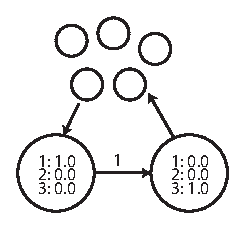
\includegraphics[width=0.45\textwidth]{images/simplemodel.eps}
\end{figure}
\textbf{When learning a simple model:}
\begin{itemize}
\item Cannot express all noise
\item May benefit more from describing general patterns
\end{itemize}
\end{frame}

\begin{frame}
\center
\begin{figure}
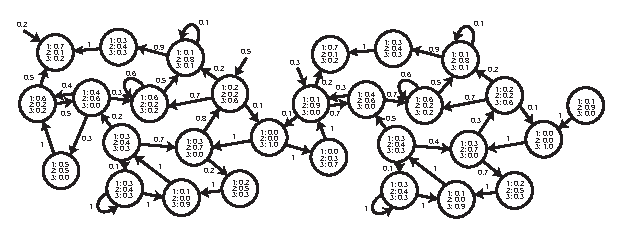
\includegraphics[width=1\textwidth]{images/complexmodel.eps}
\end{figure}
\vspace{40pt}
\textbf{When learning a complex model:}\\
\begin{itemize}
\item May be able to describe all noise
  \begin{itemize}
  \item So why not do it?
  \end{itemize}
\end{itemize}
\end{frame}

\begin{frame}
\center
How do we compare models / algorithms?
\begin{figure}
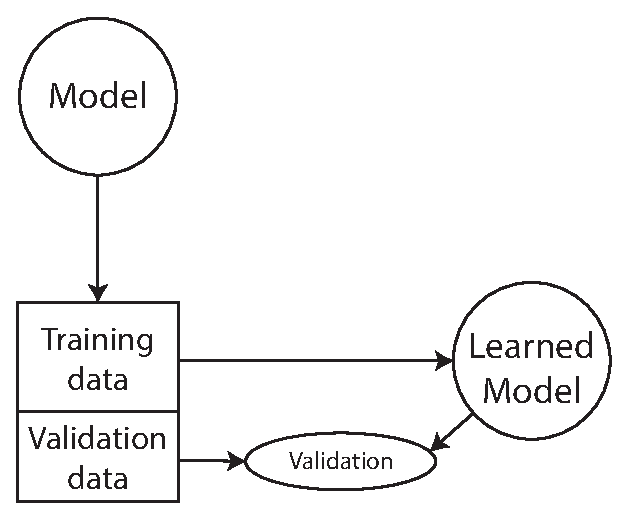
\includegraphics[width=0.7\textwidth]{images/validationdata.eps}
\end{figure}
\end{frame}

\begin{frame}
\center \huge \scshape Avoiding underflow
\end{frame}

\begin{frame}
\center
$P(X) = p_1p_2p_3p_4p_5p_6p_7p_8p_9\cdots$\\
\vspace{20pt}
$0 < p_x < 1$\\
\vspace{20pt}
Underflow when $P(X) = 0$

\end{frame}

\begin{frame}
Visual Studio, C\#: Double precision floating point
\begin{itemize}
\item $0.01^{200} = 0$
\item $0.02^{200} = 0$
\end{itemize}
Probability of a particular sequence can be very small:
\begin{itemize}
\item 23 symbols, uniformly distributed: $\frac{1}{23}^{238} = 0$
\item What about rare symbols?
\item What about probability of 1000 sequences?
\end{itemize}
\end{frame}

\begin{frame}
\center
Solution: Convert to log-space\\
$log \; (a \cdot b) = log \; a + log \; b$\\
\vspace{20pt}
Since $a < b \iff log \; a < log \; b$:\\
\vspace{20pt} 
We can often stay in Log-space
\end{frame}

\begin{frame}
\center
$log (0.01^{200}) = log \; 0.01 + log \; 0.01 + \cdots = -1381.55$\\
\vspace{20pt}
$log (0.02^{200}) = log \; 0.02 + log \; 0.02 + \cdots = -1173.60$
\end{frame}

\begin{frame}
\center
Problem: How do we sum probabilities in log space?
\end{frame}

\begin{frame}
\center
Problem: How do we sum probabilities in log space?\\
\vspace{20pt}
Solution: Scaling
\end{frame}

\begin{frame}
\begin{table}[h]
\begin{tabular}{|c|l|l|l|l|}
 \hline
Sequencee      & 1     & 3    & 3     & 2      \\ \hline
$\alpha_1(i)$          & 0.15  & 0.02 & 0.005 & 0.0007 \\ \hline
$\alpha_2(i)$          & 0.05  & 0.01 & 0.003 & 0.0005 \\ \hline
$\alpha_3(i)$          & 0.2   & 0.02 & 0.01  & 0.003  \\ \hline
\end{tabular}
\end{table}
\end{frame}

\begin{frame}
\begin{table}[h]
\begin{tabular}{|c|l|l|l|l|}
 \hline
Sequencee      & 1     & 3    & 3     & 2      \\ \hline
$\ddot{\alpha}_1(i)$          & 0.15  & 0.02 & 0.005 & 0.0007 \\ \hline
$\ddot{\alpha}_2(i)$          & 0.05  & 0.01 & 0.003 & 0.0005 \\ \hline
$\ddot{\alpha}_3(i)$          & 0.2   & 0.02 & 0.01  & 0.003  \\ \hline
Sum            & 0.4   &      &       &        \\ \hline
Scaling factor & 2.5   &      &       &        \\ \hline
$\hat{\alpha}_1(i)$          & 0.375 &      &       &        \\ \hline
$\hat{\alpha}_2(i)$          & 0.125 &      &       &        \\ \hline
$\hat{\alpha}_3(i)$          & 0.5   &      &       &        \\ \hline
\end{tabular}
\end{table}
\end{frame}

\begin{frame}
\begin{table}[h]
\begin{tabular}{|c|l|l|l|l|}
 \hline
Sequencee      & 1              & 3              & 3     & 2      \\ \hline
$\ddot{\alpha}_1$(i)          & 0.15           & \textbf{0.05}  & 0.005 & 0.0007 \\ \hline
$\ddot{\alpha}_2$(i)          & 0.05           & \textbf{0.025} & 0.003 & 0.0005 \\ \hline
$\ddot{\alpha}_3$(i)          & 0.2            & \textbf{0.05}  & 0.01  & 0.003  \\ \hline
Sum            & 0.4            & 0.125          &       &        \\ \hline
Scaling factor & 2.5            & 8              &       &        \\ \hline
$\hat{\alpha}_1(i)$          & \textbf{0.375} & 0.4            &       &        \\ \hline
$\hat{\alpha}_2(i)$          & \textbf{0.125} & 0.2            &       &        \\ \hline
$\hat{\alpha}_3(i)$          & \textbf{0.5}   & 0.4            &       &        \\ \hline
\end{tabular}
\end{table}
\end{frame}

\begin{frame}
\begin{table}[h]
\begin{tabular}{|c|l|l|l|l|}
 \hline
Sequencee      & 1     & 3            & 3             & 2      \\ \hline
$\ddot{\alpha}_1(i)$          & 0.15  & 0.05         & \textbf{0.32} & 0.0007 \\ \hline
$\ddot{\alpha}_2(i)$          & 0.05  & 0.025        & \textbf{0.2}  & 0.0005 \\ \hline
$\ddot{\alpha}_3(i)$          & 0.2   & 0.05         & \textbf{0.01} & 0.003  \\ \hline
Sum            & 0.4   & 0.125        & 0.53          &        \\ \hline
Scaling factor & 2.5   & 8            & 1.89          &        \\ \hline
$\hat{\alpha}_1(i)$          & 0.375 & \textbf{0.4} & 0.604         &        \\ \hline
$\hat{\alpha}_2(i)$          & 0.125 & \textbf{0.2} & 0.378         &        \\ \hline
$\hat{\alpha}_3(i)$          & 0.5   & \textbf{0.4} & 0.018         &   	   \\ \hline    
\end{tabular}
\end{table}
\end{frame}

\begin{frame}
\begin{table}[h]
\begin{tabular}{|c|l|l|l|l|}
\hline
Sequencee      & 1     & 3     & 3              & 2                 \\ \hline
$\ddot{\alpha}_1(i)$          & 0.15  & 0.05  & 0.32           & \textbf{0.001323} \\ \hline
$\ddot{\alpha}_2(i)$          & 0.05  & 0.025 & 0.2            & \textbf{0.000945} \\ \hline
$\ddot{\alpha}_3(i)$          & 0.2   & 0.05  & 0.01           & \textbf{0.00567}  \\ \hline
Sum            & 0.4   & 0.125 & 0.53           & 0.007938          \\ \hline
Scaling factor & 2.5   & 8     & 1.89           & 125.98            \\ \hline
$\hat{\alpha}_1(i)$          & 0.375 & 0.4   & \textbf{0.604} & 0.167             \\ \hline
$\hat{\alpha}_2(i)$          & 0.125 & 0.2   & \textbf{0.378} & 0.119             \\ \hline
$\hat{\alpha}_3(i)$          & 0.5   & 0.4   & \textbf{0.018} & 0.714             \\ \hline  
\end{tabular}
\end{table}
\end{frame}
\subsection{Algorithms}
In this section a number of algorithms are described, which all try to learn the parameters of a \gls{hmm} given a set of training sequences $D$, which contains a number of sequences over $s$ distinct symbols.
In other words, each algorithm will try to find a model that makes the generation of the particular training sequences most likely.
Since a \gls{hmm} can be represented by the use of either matrices or a graph like structure, any of the algorithms may output either a matrix or graph representation of a \gls{hmm}, denoted by $M$ or $G$ respectively.
By $LL(M)$ or $LL(G)$ we denote the likelihood of the training sequences given the model.

The algorithms proposed in this section have been divided into two types.
The static algorithms start with a \gls{hmm} with a particular number of states which will never change.
The dynamic algorithms start with a \gls{hmm} of just a single state, and will dynamically extend the number of states through a number of iterations. 
For the static algorithms, $n$ denotes the number of states to be used.
The dynamic algorithms will by $n$ denote a number of iterations $1, ..., n$, where each iteration extends the model by a single node.
In \ref{fig:alg-hierarchy} the names and classes of our proposed algorithms can be seen. Note that the Baum Welch algorithm has also been included, simply to emphasize which class of algorithms it belongs to. 

\begin{figure}
\label{fig:alg-hierarchy}
\caption{The algorithms used in our experiments}
\Tree[.Algorithms
		[.{Static size} 
			{Baum Welch}
            {Sparse Baum Welch}
        ]
       	[.{Dynamic size} 
       		{Strict George}
       		{George}
       		{Greedy Extend}
      	]
     ]
\end{figure}

Since the Baum Welch algorithm is guaranteed to never worsen $LL(G)$ when run on $G$, it is used internally by some of the algorithms.
By $BW_t(M, D)$ we denote the \gls{hmm} obtained after running Baum Welch on the \gls{hmm} $M$ using the training sequences $D$, and iterating as long as each iteration increases the likelihood by at least $t$.
By $BW^i(M, D)$ we denote the \gls{hmm} obtained after running $i$ iterations of Baum Welch on the \gls{hmm} $M$ using the training sequences $D$.
If a \gls{hmm} is represented by a graph, we denote it $G$, and the similar notations $BW_t(G, D)$ and $BW^i(G, D)$ are used.


\subsection{Greedy Extend}
Initially, a graph representation $G$ of a single state \gls{hmm} is created. The single node has initial probability 1, loops to itself with probability 1, and its emission probabilities for each of the $s$ symbols are chosen randomly and normalised.

The following pseudo code describes how the algorithm continuously tries to extend the graph, as long as it improves the likelihood of the data:

\begin{itemize}
\item (1) Repeat $\alpha$ times:
	\begin{itemize}
	\item $G'$ = $(V(G) \cup \{y'\}, E(G))$, where $y'$ is a new node with a random initial probability in range $[0, 1]$ having random emission probabilities for all $s$ symbols, which sums to $1$.
	\item Randomly choose a set of nodes $Y = \{y_1, y_2, ... , y_l\}$ from $V(G')$, where $l = \lceil \log |V(G')| \rceil$ and $\forall a,b: y_a \neq y_b$.
	\item For each $y \in Y$, the transitions $(y, y')$ and $(y', y)$ are added to $E(G')$ with random transition probabilities.
	\item Normalize $G'$.
	\item If $LL(BW^{\beta}(G', D)) > LL(G)$, let $G = LL(BW^{\beta}(G', D))$, go to (1).
	\begin{itemize}
		\item Return $BW_t(G, D)$.
	\end{itemize}
	\end{itemize}
\end{itemize}

\paragraph{Determining the $\alpha$ Value}

The value $\alpha$ determines how many times the algorithm will try to expand the model. If the $\alpha$ attempts cannot improve the model further, it stops and returns the model. By observing the algorithm it is clear that most small model improve with the very first expansion attempt, while larger models need more attempt to find a new state that improves the model. It is difficult to determine exactly how many expansion attempt that can be deemed sufficient, as the amount of random expansion possibilities is very large, however as we shall see later in Chapter \ref{chap:experiment} where 100 runs were used, only few experiments ended because 100 expand attempts without improving.

\paragraph{Determining the $\beta$ Value}

Another big question about the Greedy Extend algorithm, is how the choice of $\beta$ affects the performance of the algorithm.
As $\beta$ denotes the number of Baum Welch iterations to run each time the algorithm attempts to extend the graph, increasing $\beta$ will also increase the run time of the algorithm. It may be the case that better results are achieved when $\beta$ is increased, since more iterations of Baum Welch also means a greater increase in likelihood. However, it could be the case that using many iterations early increases the chance of getting trapped in a local optimum.
An experiment has been conducted of using different values for $\beta$ on data set $1$ from the Pautomac competition. The results can be seen in figure \ref{fig:ge-different-thresholds-tested}. Each line represents the mean value of 5 runs of the Greedy Extend algorithm with the specified number of iterations. Some of the plots have been cut off at a point where one of the runs did not manage to extend beyond a certain number of states.

\begin{figure}[!h]
\begin{centering}
\begin{tikzpicture}
	\pgfplotsset{every axis legend/.append style={ 
		at={(0.5,1.06)},
		anchor=south}}
	\begin{axis}[
			scale = 1.5,
			xlabel = Number of states,
            	ylabel = Score (lower is better),
            	legend columns=-1,
            	legend entries={IT-0, IT-1, IT-2, IT-3, IT-5, IT-10, IT-50},
			legend style={/tikz/every even column/.append style={column sep=0.3cm}}]
		
		\addplot+[mark=none]table[x=States, y=IT-0, col sep=tab]
		{content/Models/Algorithms/ge-intermediate-iterations-test.csv};
		
		\addplot+[mark=none]table[x=States, y=IT-1, col sep=tab]
		{content/Models/Algorithms/ge-intermediate-iterations-test.csv};
		
		\addplot+[mark=none]table[x=States, y=IT-2, col sep=tab]
		{content/Models/Algorithms/ge-intermediate-iterations-test.csv};
		
		\addplot+[mark=none]table[x=States, y=IT-3, col sep=tab]
		{content/Models/Algorithms/ge-intermediate-iterations-test.csv};

		\addplot+[mark=none]table[x=States, y=IT-5, col sep=tab]
		{content/Models/Algorithms/ge-intermediate-iterations-test.csv};
		
		\addplot+[mark=none]table[x=States, y=IT-10, col sep=tab]
		{content/Models/Algorithms/ge-intermediate-iterations-test.csv};
		
		\addplot+[mark=none]table[x=States, y=IT-50, col sep=tab]
		{content/Models/Algorithms/ge-intermediate-iterations-test.csv};
	\end{axis}
\end{tikzpicture} 
\caption{Test of different values for $\beta$ while running the Greedy Extend algorithm.}
\label{fig:ge-different-thresholds-tested} 
\end{centering}
\end{figure}

The figure shows surprisingly that using no iterations is somehow better than using just a single iteration. However, using 5 or more iterations is better than not using any iterations at all.
When using 5 iterations, only a single run did not reach 50 states (it stopped at 49).
We later choose to conduct further experiments with $\beta = 10$, since all runs with 10 iterations reached 50 states, and it looks like the performance does not change significantly when increasing the number of iterations beyond 10.
\subsection{Sparse Baum Welch}
This algorithm creates a \gls{hmm} $M$ with $n$ states and $s$ symbols.
All parameters are initialized randomly but with the constraint that each state has exactly $\lceil log(n) \rceil$ outgoing transitions.
Which transitions to discard are chosen randomly before training with \gls{baum-welch} either by $BW_t(M, D)$ or $BW^i(M, D)$.
\subsection{State Splitting Approach}

Another dynamic size \gls{hmm} learning approach was to construct a greedy heuristics to ``split'' states. Several versions and concepts were attempted whilst maintaining the \gls{baum-welch} as a basis for the approach, running it repeatedly on the growing model to ensure convergence. The initial experiments were splitting states until a given number of states ($n$) was reached, but a threshold ($\theta$) mechanic was employed at a later time in attempt to reduce the dependency on the prior knowledge of number of states.

The greedy state splitting algorithm consists of two main modules, with possible extensions. The main modules include the heuristics to identify the state (or multiple states) to split and the splitting algorithm itself. During the experiments, two additional concepts, not fundamental for the state splitting itself, were also explored - edge cutting and state removal.

\subsubsection{State Split Mechanics}
Two main approaches to splitting the states were considered for the state splitting algorithm. One being very simple, just producing a copy of the state to split (\emph{Clone split}) and a much more elaborate approach considering the topology of the state inside the hidden state graph (\emph{Distribution split}).

\subsubsection{State Identification Heuristics}
Similarly to state splitting itself, two main approaches were explored for identifying the best state to split. The first one utilised the \gls{viterbi} thus named the \emph{Viterbi heuristic}, whilst the second one uses the $\gamma_t(i)$ variables computed during the \gls{baum-welch} algorithm and was therefore named the \emph{Gamma heuristic}.

Both of the heuristics compute a score $\zeta:S \rightarrow \mathcal{R}$ for each hidden state of the model, that can later be utilised to determine the state to split.

\paragraph{Viterbi Heuristic}
The \emph{Viterbi heuristic} computes the score $\zeta$ for each hidden state as a probability of producing the correct symbol in the validation sequences for which it belongs to the corresponding most probable hidden state sequence as determined by the \gls{viterbi}.

In more formal terms, the computation of the score $\zeta(s)$ for each $s \in S$ and a given \gls{hmm} $\lambda = (\mathbf{A}, \mathbf{B}, \boldsymbol{\pi})$ can be described by the following procedure:
\begin{enumerate}
	\item For each signal $\mathbf{O}\in V$ a corresponding most probable hidden state sequence is computed using the \gls{viterbi}: $\mathbf{Q}=\mathcal{V}_G(\mathbf{O})$.
	\item For each state $s\in S$ determine the significant positions in the hidden state sequences given by \gls{viterbi}:
	$$\forall s\in S,\forall \mathbf{O}=(o_1, ..., o_T)\in V: \tau_{s, \lambda}^\mathbf{O}=\{t\in\{1, ..., T\}|\mathbf{Q}_t=s\}$$
	\item For each state $s \in S$  and $\mathbf{O}\in V$ compute the partial score (performance) $\hat\zeta_{\mathbf{O}}(s)$ as the average probability of producing the expected observable symbol in accordance to the signal $\mathbf{O}$ over all the significant positions for the given state $s$ and signal $\mathbf{O}$:
	$$\forall s\in S,\forall \mathbf{O}\in V: \hat{\zeta}_{\mathbf{O}}(s) = \frac{\sum_{t\in\tau_{s, \lambda}^{\mathbf{O}}}b_s(o_t)}{|\tau_{s, \lambda}^{\mathbf{O}}|}$$
	\item Finally, compute the $\zeta$ score for each state $s\in S$ as a sum of all the partial scores for the given state weighted by the probabilities of generating the associated signals by the corresponding hidden state sequences:
	$$\forall s\in S: \zeta(s)=\sum_{\mathbf{O}\in V}P(\mathbf{Q}|\mathbf{O}, \lambda)\hat\zeta_{s, \lambda}^{\mathbf{O}}$$
\end{enumerate}

The obtained $\zeta$ scores the states of the \gls{hmm} based on their ``performance'' for the tasks they are most likely to perform. As such the state with the lowest score is determined to be the worst performing node $w$: $$w = \argmin_{s\in S}(\zeta(s))$$

This node is deemed to be the worst performing one as a result of being involved in the generation of many of the signals in the validation set $V$. As such, it seems meaningful to split the node into two, in order to share the extensive workload and increase performance.

The \emph{Viterbi heuristic} can be straightforwardly extended to identify more than just one state to split, thereby producing a set of the worst performing nodes $\mathcal{W}$. The set can be constructed iteratively starting with $\mathcal{W} = \emptyset$ as:
$$\mathcal{W} = \mathcal{W} \cup \{\argmin_{s\in S\setminus \mathcal{W}}(\zeta(s))\}$$
until the $|\mathcal{W}|$ equals the desired number of states to split.

A further modification of the \emph{Viterbi heuristic} was considered to incorporate the use of a splitting threshold $\theta$ instead of a maximum number of states. For this purpose a normalised version of the score $\overline{\zeta}$ was introduced:
$$\overline{\zeta}(s) = \frac{\zeta(s)}{\sum_{s\in S}\zeta(s)}$$

The states to split $\mathcal{W}$ were thus determined as all states that scored below the given threshold $\theta$:
$$\mathcal{W} = \{s\in S|\overline\zeta(s) < \theta\}$$

More improvements to the \emph{Viterbi heuristic} were considered, mainly including the \emph{n-step Viterbi heuristic} that would have computed the score on not only the output probability in the given significant position, but also on the probability of correctly outputting the next $n -1$ symbols of the given signal - starting from the explored state - to further increase precision. The above described version of the \emph{Viterbi heuristic} would be considered \emph{1-step Viterbi heuristic} in this context. This approach however remains untested due to preference of the \emph{Gamma heuristic} and can be considered for future work.

\paragraph{Gamma Heurisitic}

\todo{Finish the state splitting section.}

%This algorithm utilises a greedy concept to grow the hidden state space of a \gls{hmm} whilst maintaining a sparse transition matrix to preserve computability in large state spaces. The Greedy %State Splitting relies heavily on the existing \gls{baum-welch} calling it repeatedly to achieve convergence.

%Let $(n, s, \epsilon, D, V)$ be the input vector of the Greedy State Splitting algorithm where: $n, s \in \mathbb{N}, \epsilon\in[0,1], D$ is the training data set and $V$ is the validation data %set. The greedy State Splitting algorithm starts with two vertex complete graph $G=K_2$ for the hidden state space with all the parameters randomised. Afterwards it iterates through the %following phases until $|V(G)| = n$:

%\begin{itemize}
%	\item[] Phase 1, state splitting
%	\item[1)] For each observable state sequence $\mathbf{O} \in V$ a corresponding most probable hidden state sequence is computed using \gls{viterbi}: %$\mathbf{Q}=\mathcal{V}_G(\mathbf{O})$.
%	\item[2)] For each vertex $v \in V(G)$ compute a score $s(v)$ as the probability the given vertex outputs the desired output symbol according to the precomputed hidden state %sequences weighted by the probability of these sequences. In more formal terms, let $\theta_G(\mathbf{O}=(o_1,...,o_T), v) = \{t\in\{1, ..., T\}|\mathbf{Q}_t=v\}$ then: $$s(v) = %\sum_{\mathbf{O}\in V}P(\mathbf{Q}|\mathbf{O},G) \frac{\sum_{t \in \theta_G(\mathbf{O}, v)}b_v(o_t)}{|\theta_G(\mathbf{O}, v)|}$$
%	\item[3)] Find the ``weakest'' vertex: $$w = \argmin_{v\in V(G)}\{s(v)\}$$.
%	\item[4)] Create a new graph $G' = G\cup \{w'\}$ where $w'$ is a new vertex such that: $\forall v\in V(G): a_{w'v} = a_{wv} \land a_{vw'} = a_{vw}$, $\forall \sigma \in \Sigma: %b_{w'}(\sigma) = b_w(\sigma)$ and $\pi(w') = \pi(w)$.
%	\item[5)] Normalise $G'$ so all the probabilities sum up to $1$.
%	\item[] Phase 2, edge cutting
%	\item[6)] For each edge $e = (v_1,v_2)\in E(G')$ check if the edge probability is lower then the given threshold: $a_{v-1,v_2}<\epsilon$. If so, remove the edge from the graph %($a_{v-1,v_2} = 0$).
%	\item[] Phase 3, re-estimation of the model parameters.
%	\item[7)] Run \gls{baum-welch} to re-learn the model parameters of the new model: $G = BW_t(G', D)$.
%\end{itemize}

%The algorithm has also been considered in a ``strict'' variation at first, where the edge cutting phase did not depend on the parameter $\epsilon$ but instead a constant out-degree was %maintained for all vertices, namely the size of the output symbol alphabet $s = |\Sigma|$. The early results however showed, that the strict out-degree variation is outperformed by the %$\epsilon$ threshold.
\subsubsection{Gamma State Splitting}

% finding the most used state for a given sentence.
$$q' = \argmax_{q \in Q}\sum_{o \in O}\sum_{t=0}^{T}\gamma_t(q)$$ 

% find all possible transitions from q'
$$z = \{a_{q'J} \in A \vert a_{q'J} \neq 0\}$$

% compute average transition probability
$$z_{arg} = \frac{\sum_{a_{q'J} \in z} a_{q'J}}{\vert z \vert}$$

% compute the absolute error sum of all transitions. 
$$AbsE = \sum_{a_{q'J} \in z} \vert a_{q'J} - z_{arg} \vert$$

% if the absolute error is below the threshold value epsilon the
% distribution is fairly uniform and the state q' is split into q_1 and q_2.
$$Q' = \begin{cases}
	Q-\{q'\} \cup \{ q_1,q_2 \} &\text{if } AbsE > \epsilon_1 \\
	Q	&\text{otherwise}
\end{cases}$$

% 
$$A_1 = \{a_{q_1i} \vert a_{q_1i} = a_{q'i} \wedge a_{q'i} \in A \wedge a_{q'i} >0 \wedge i \in Q' - \{q_1\}\}$$

$$A_2 = \{a_{q_2i} \vert a_{q_2i} = a_{q'i} \wedge a_{q'i} \in A \wedge a_{q'i} > 0 \wedge i \in Q' - \{q_2\}\}$$

$$A_1 \cap A_2 = \emptyset$$

$$\vert A_1 \vert = \vert A_2 \vert$$

$$A' = A_1 \cup A_2$$

$$\sum_{a_{q_1i} \in A_1} a_{q_1i} = \sum_{a_{q_2J} \in A_1} a_{q_1J}$$

$$A_1 = \{a_{q_1i} \vert a_{q_1i} \in A \wedge a_{q_1i} \notin A_2\}$$
	$$A_1 = \{a_{q_2i} \vert a_{q_2i} \in A \wedge a_{q_2i} \notin A_1\}$$





\section{\scshape Experiment Setup}

%\begin{frame} 
%\center \huge \scshape Test Environment
%\end{frame}

%\begin{frame}
%  \frametitle{Test Environment}
%  \begin{itemize}
%		\item Benchmark
%		\item Data
%	  	\item PautomacEvaluator
%	  	\item Learner
%	  	\item Models
%  \end{itemize}
%\end{frame}

\begin{frame}
	\center \huge \scshape Selecting Dataset
\end{frame}

\begin{frame}
	\frametitle{Dataset}
	\begin{itemize}
		\item 48 to 12 Datasets
		\item Number of States
		\item Transition Density
		\item Number of Symbols
	\end{itemize}
\end{frame}

\begin{frame}
	\frametitle{Number of States}
		\begin{centering}
			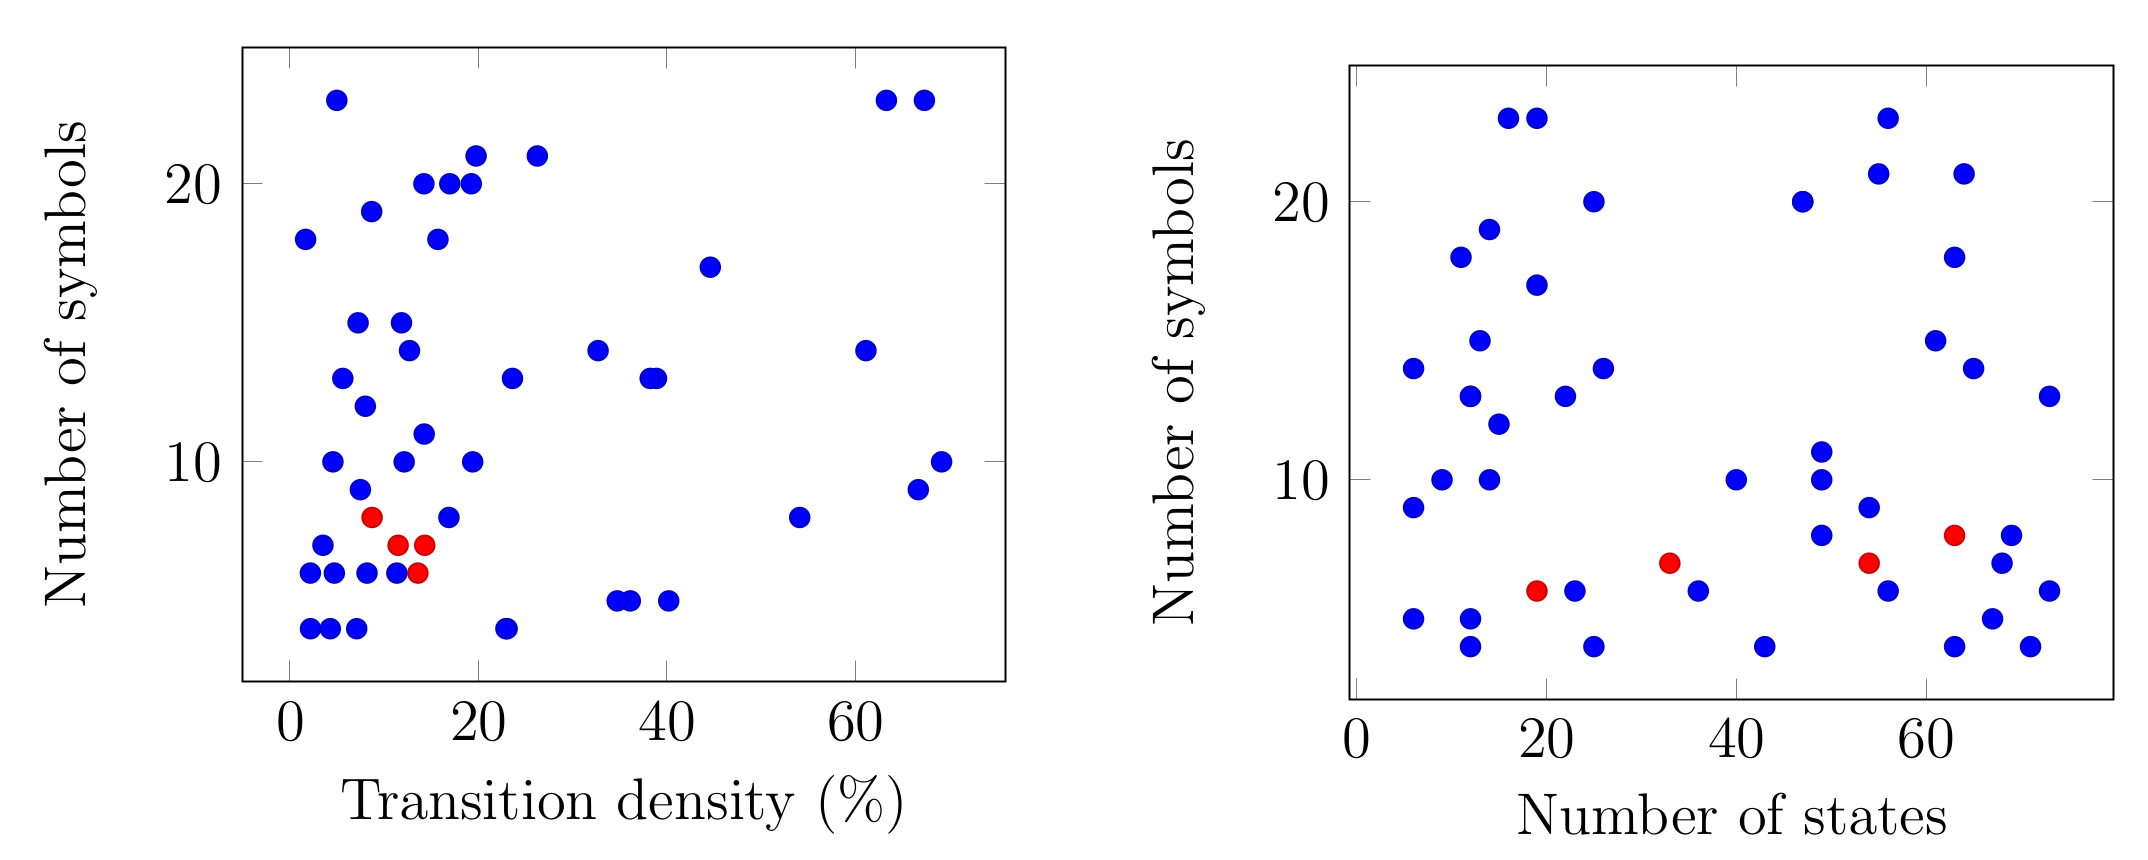
\includegraphics[width=1\textwidth]{images/states.png}
		\end{centering}
\end{frame}

\begin{frame}
	\frametitle{Transition Density}
	Ratio between number of transitions and total number of possible transitions in the model
	\begin{centering}
		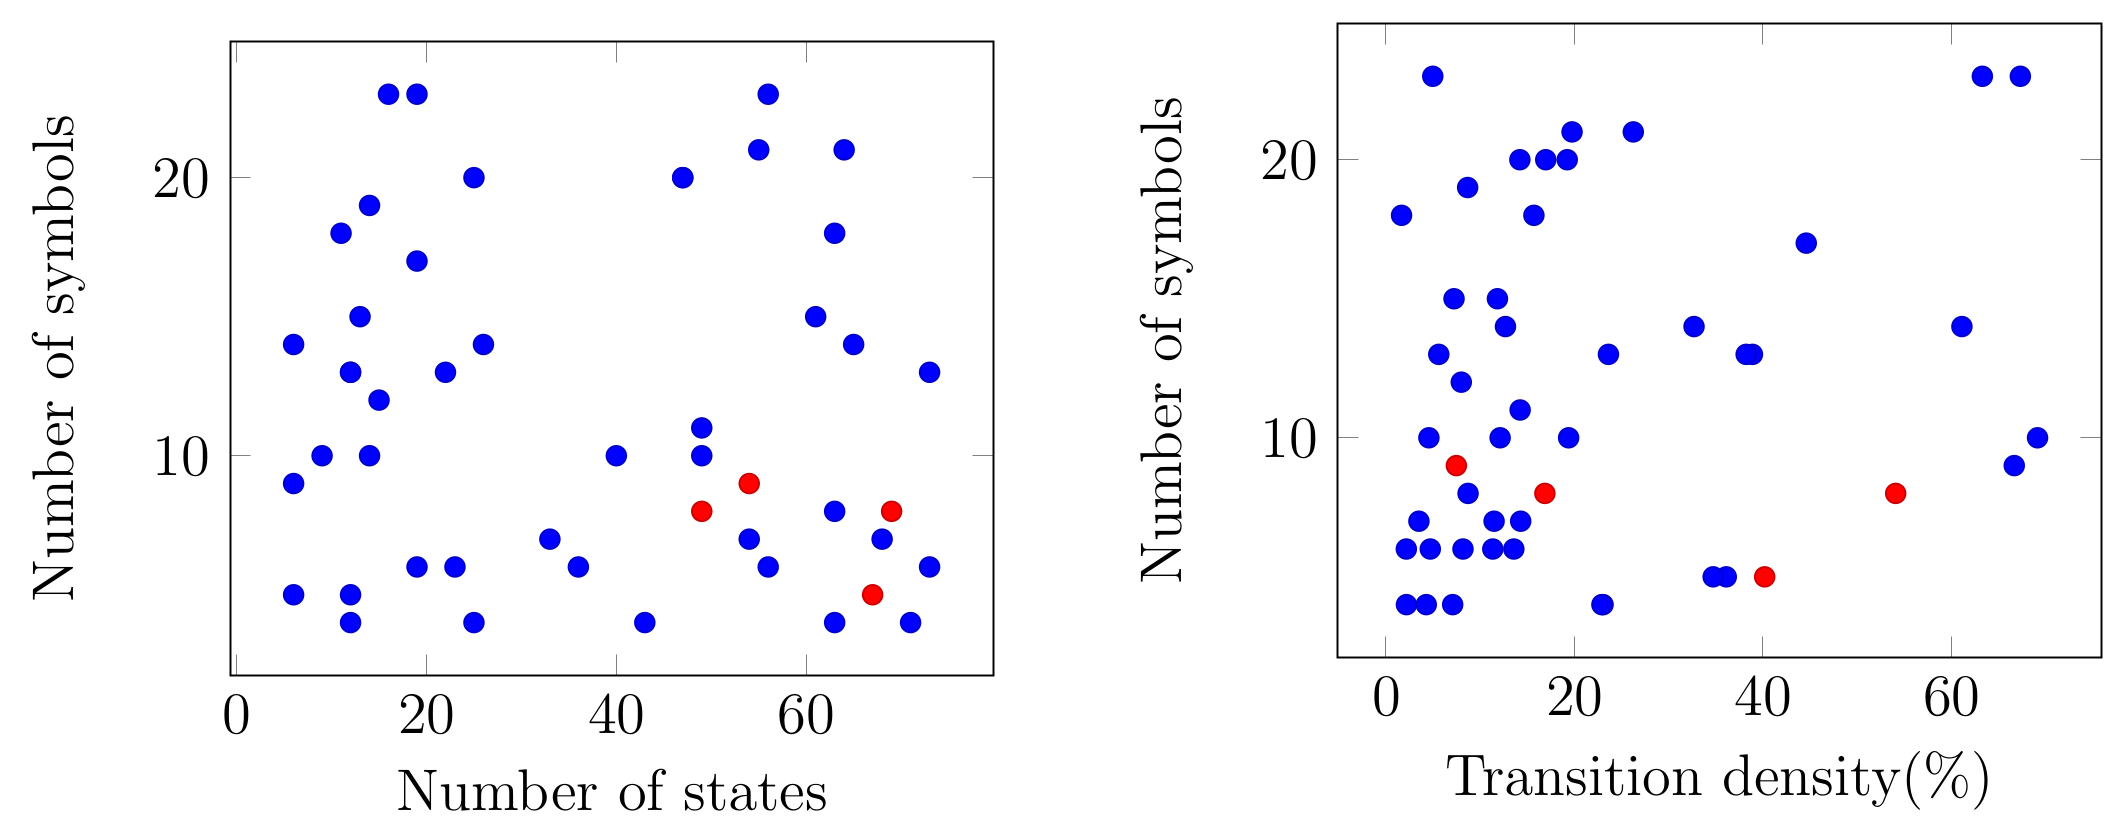
\includegraphics[width=1\textwidth]{images/transition.png}
	\end{centering}
\end{frame}

\begin{frame}
	\frametitle{Number of Symbols}
	\begin{centering}
		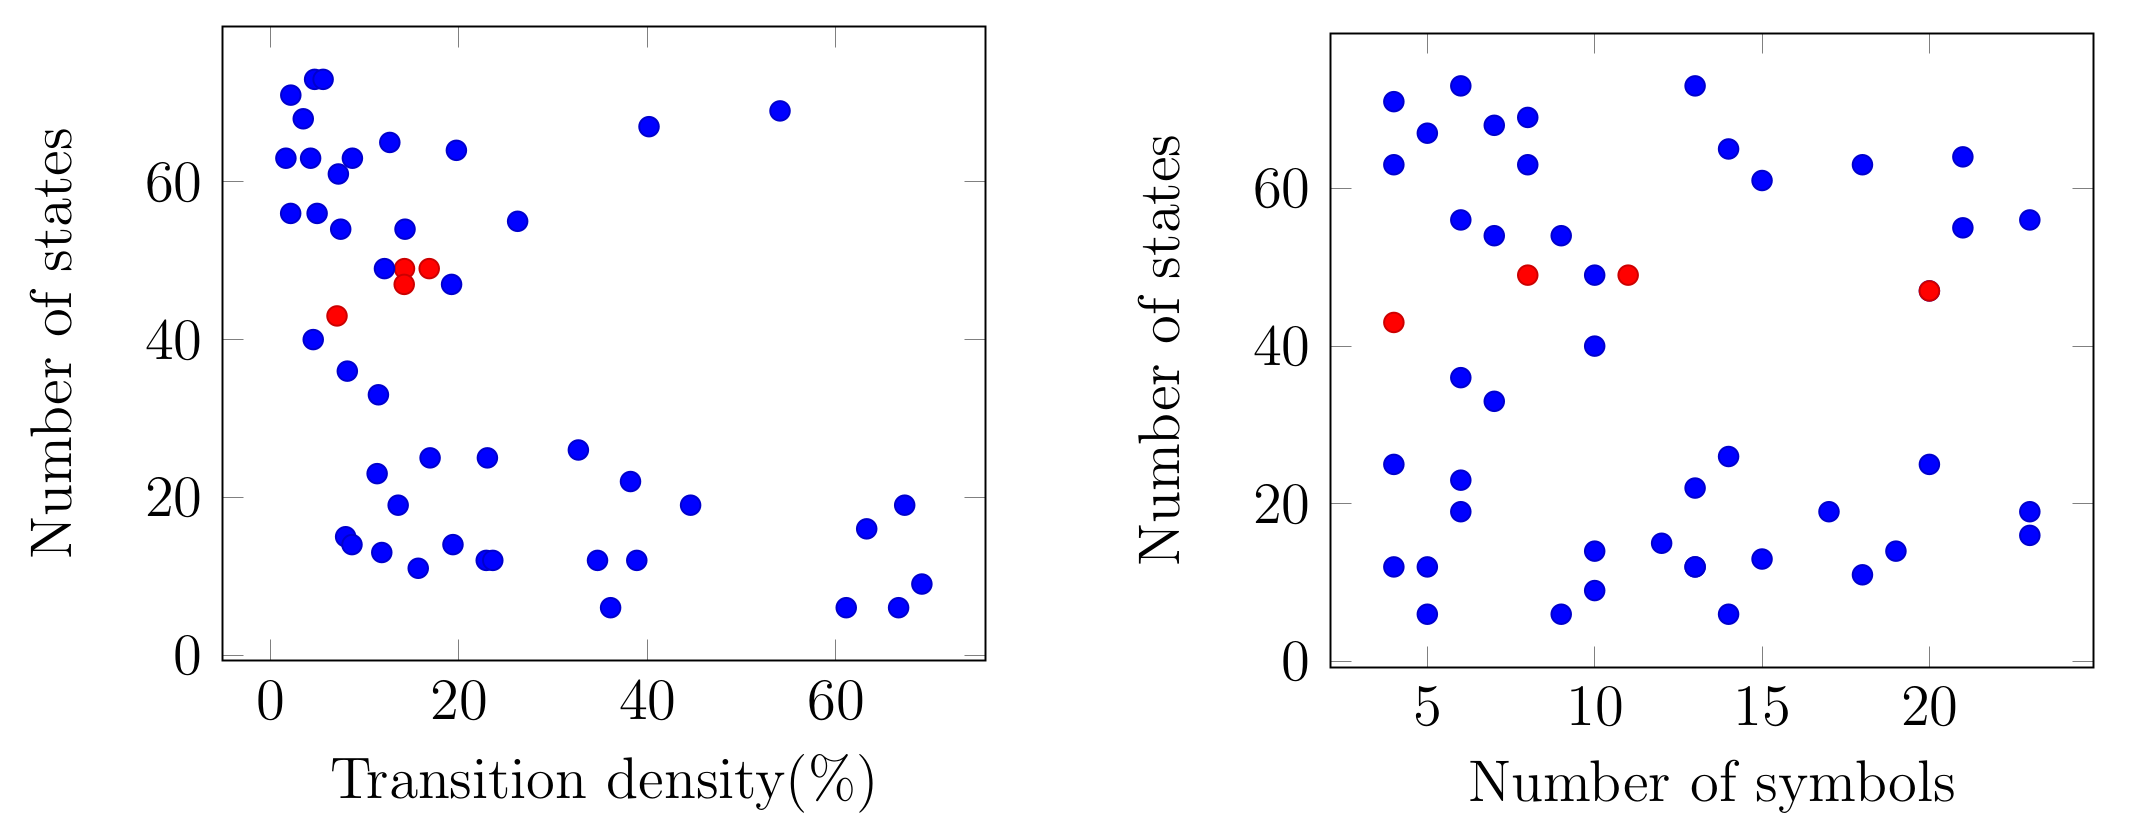
\includegraphics[width=1\textwidth]{images/symbols.png}
	\end{centering}
\end{frame}

\begin{frame}
	\frametitle{Datasets}
	\begin{centering}
		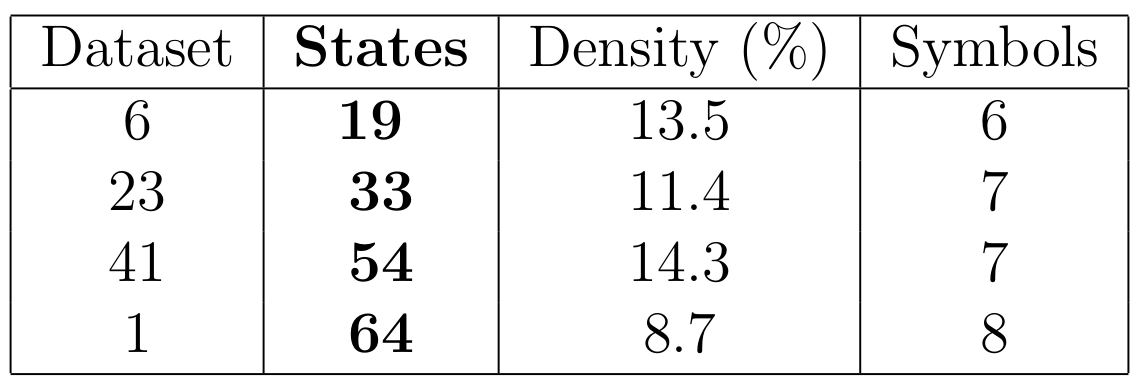
\includegraphics[width=0.7\textwidth]{images/table1.png}\\
		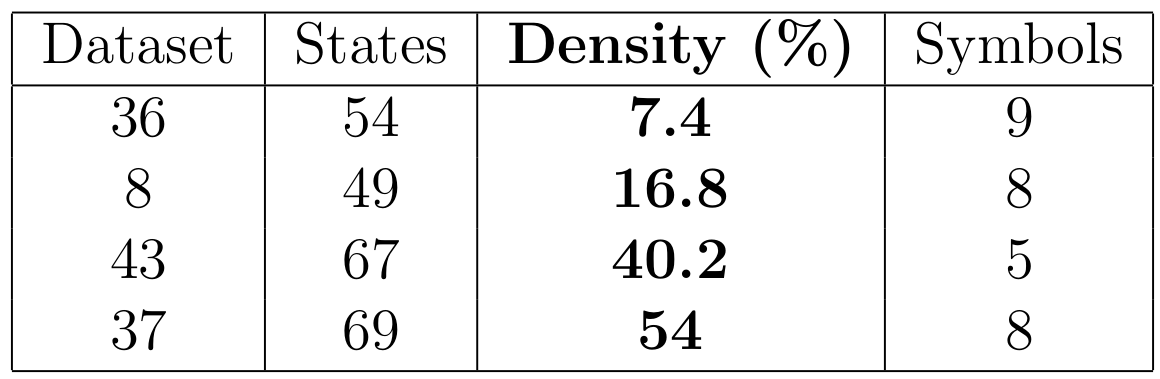
\includegraphics[width=0.7\textwidth]{images/table2.png}\\
		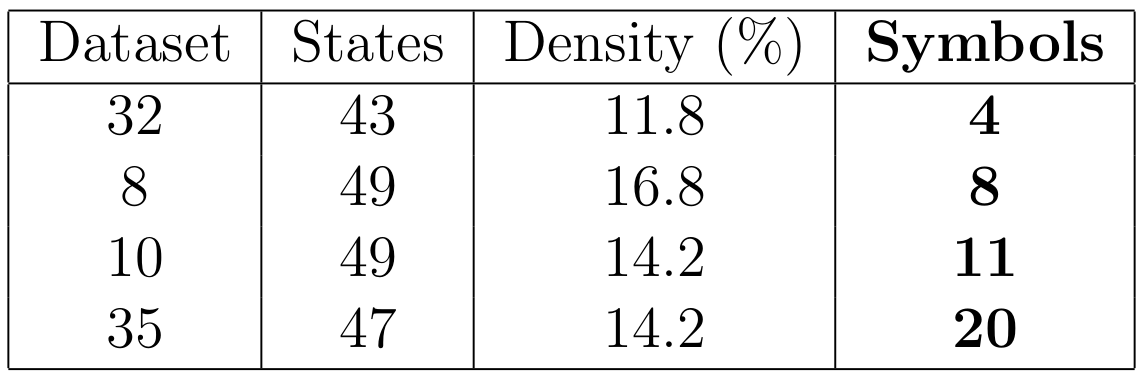
\includegraphics[width=0.7\textwidth]{images/table3.png}\\
	\end{centering}
\end{frame}

% % % % % % % % % % % % % % % % % % % % % % % % % % % % % % % %

\begin{frame}
	\center \huge \scshape Experiment Parameter
\end{frame}

\begin{frame}
	\frametitle{Experiment Parameter}
	\begin{itemize}
		\item Static Learners
		\item Training Sequences
		\item Baum-Welch Threshold
		\item Greedy Extend
	\end{itemize}
\end{frame}


\begin{frame}
	\frametitle{Static Learners}
	\begin{itemize}
		\item Baum-Welch input
		\item States for the HMM
		\item Threshold
		\item Maximum 73 states
		\item 10 to 100 step 10
	\end{itemize}
\end{frame}


\begin{frame}
	\frametitle{Training Sequences}
		\begin{itemize}
			\item 100 to 50000
			\item Baum Welch
			\item Dataset 36
			\item Threshold = 0.01
			\item States = 
		\end{itemize}
\end{frame}

\begin{frame}
	\frametitle{Training Sequences}
	\begin{itemize}
		\item 5000 Sequences
	\end{itemize}
	\begin{centering}
		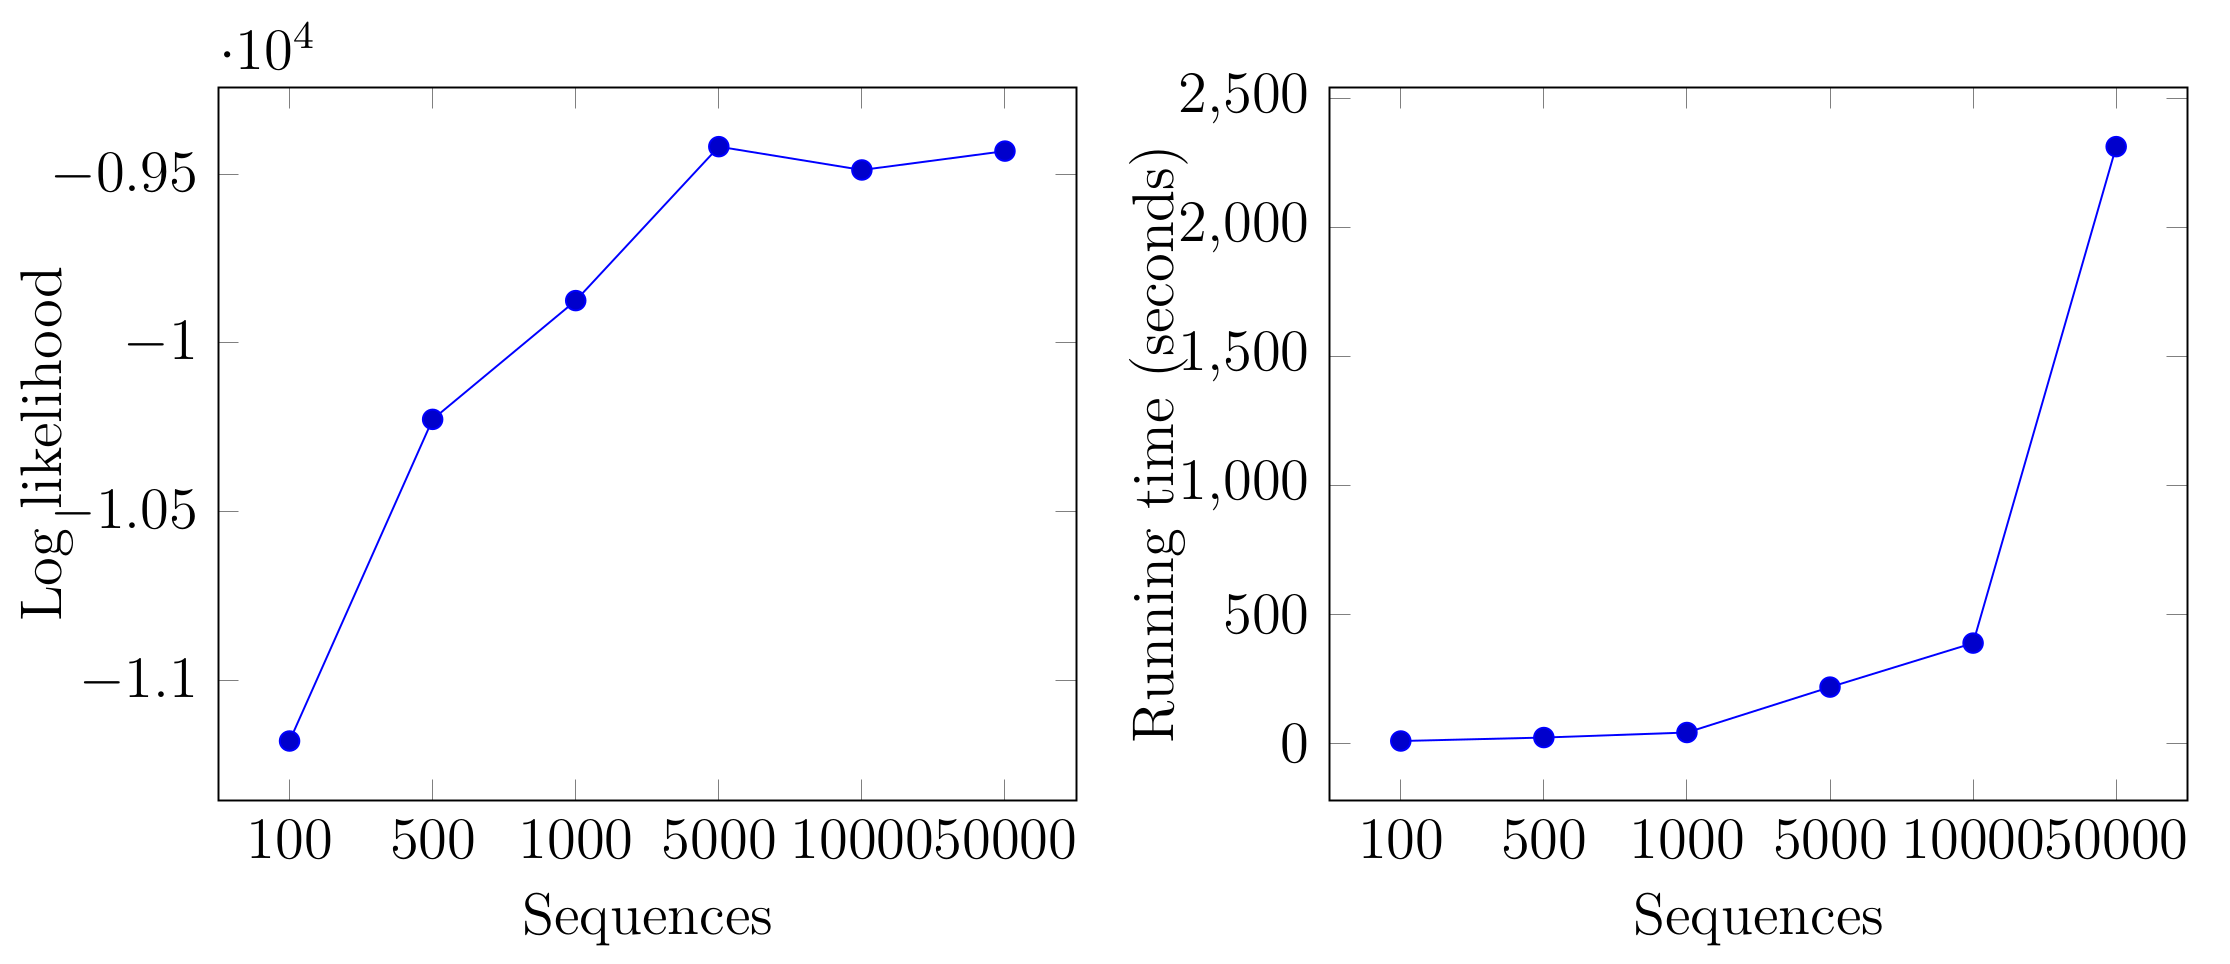
\includegraphics[width=1\textwidth]{images/sequences.png}
	\end{centering}
\end{frame}

\begin{frame}
	\frametitle{Baum-Welch Threshold}
	\begin{columns}[t]
		\begin{column}{3.3cm}
			\begin{itemize}
				\item Static value
				\item 50 states
				\item 0.1 to 0.0001
				\item Threshold 0.01
			\end{itemize}
		\end{column}
		\begin{column}{12cm}
			\begin{flushleft}			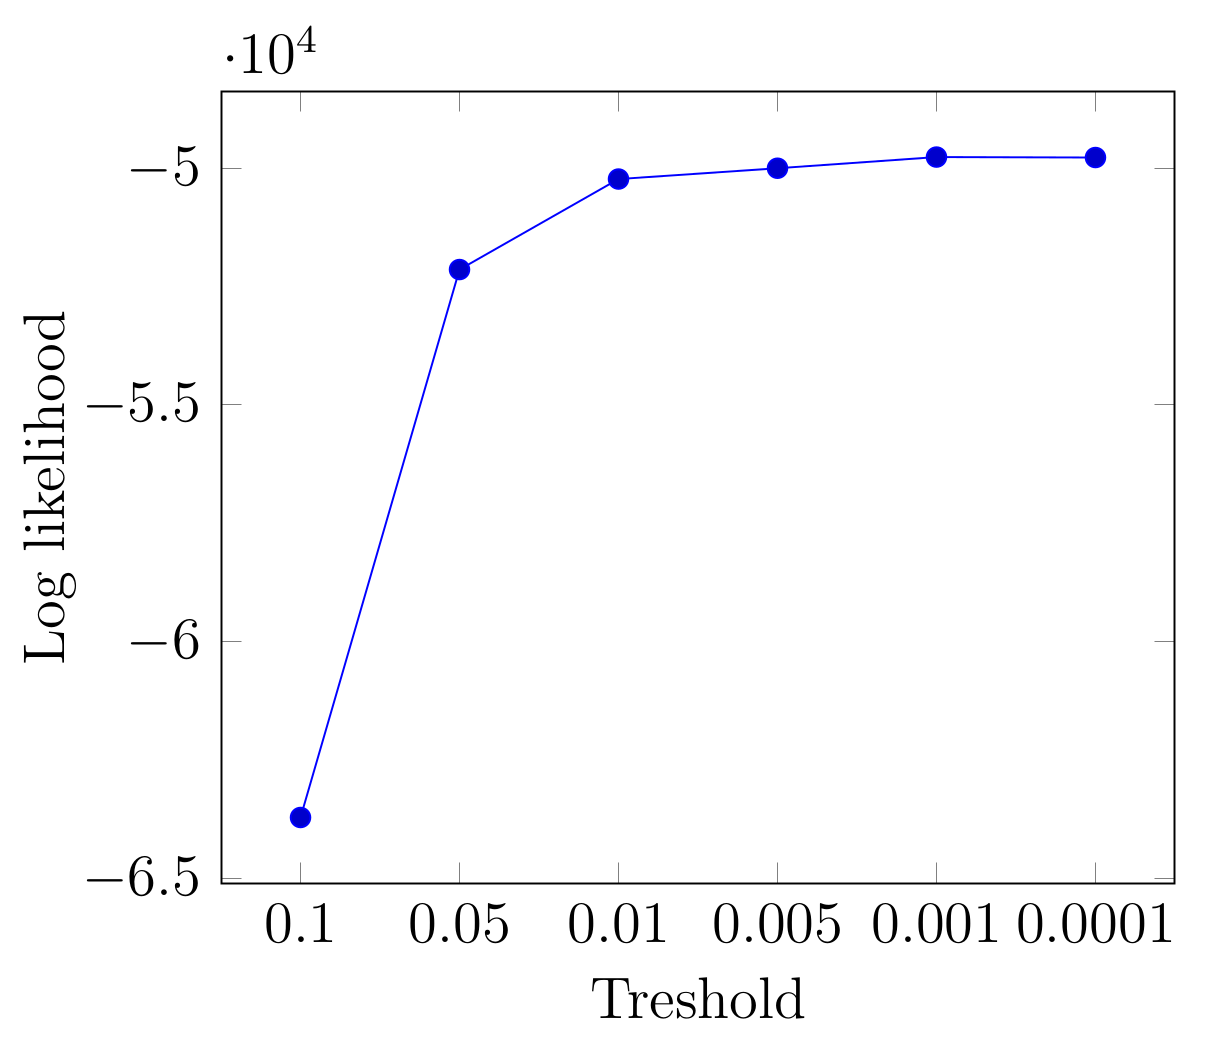
\includegraphics[width=0.7\textwidth]{images/threshold.png}
			\end{flushleft}
		\end{column}
	\end{columns}
	
\end{frame}

\begin{frame}
	\frametitle{Greedy Extend}
	\begin{itemize}
		\item $\beta$-value
		\item Baum-Welch iteration
		\item Running time
		\item Local optimum
	\end{itemize}
\end{frame}

\begin{frame}
	\frametitle{Greedy Extend}
	\begin{centering}
		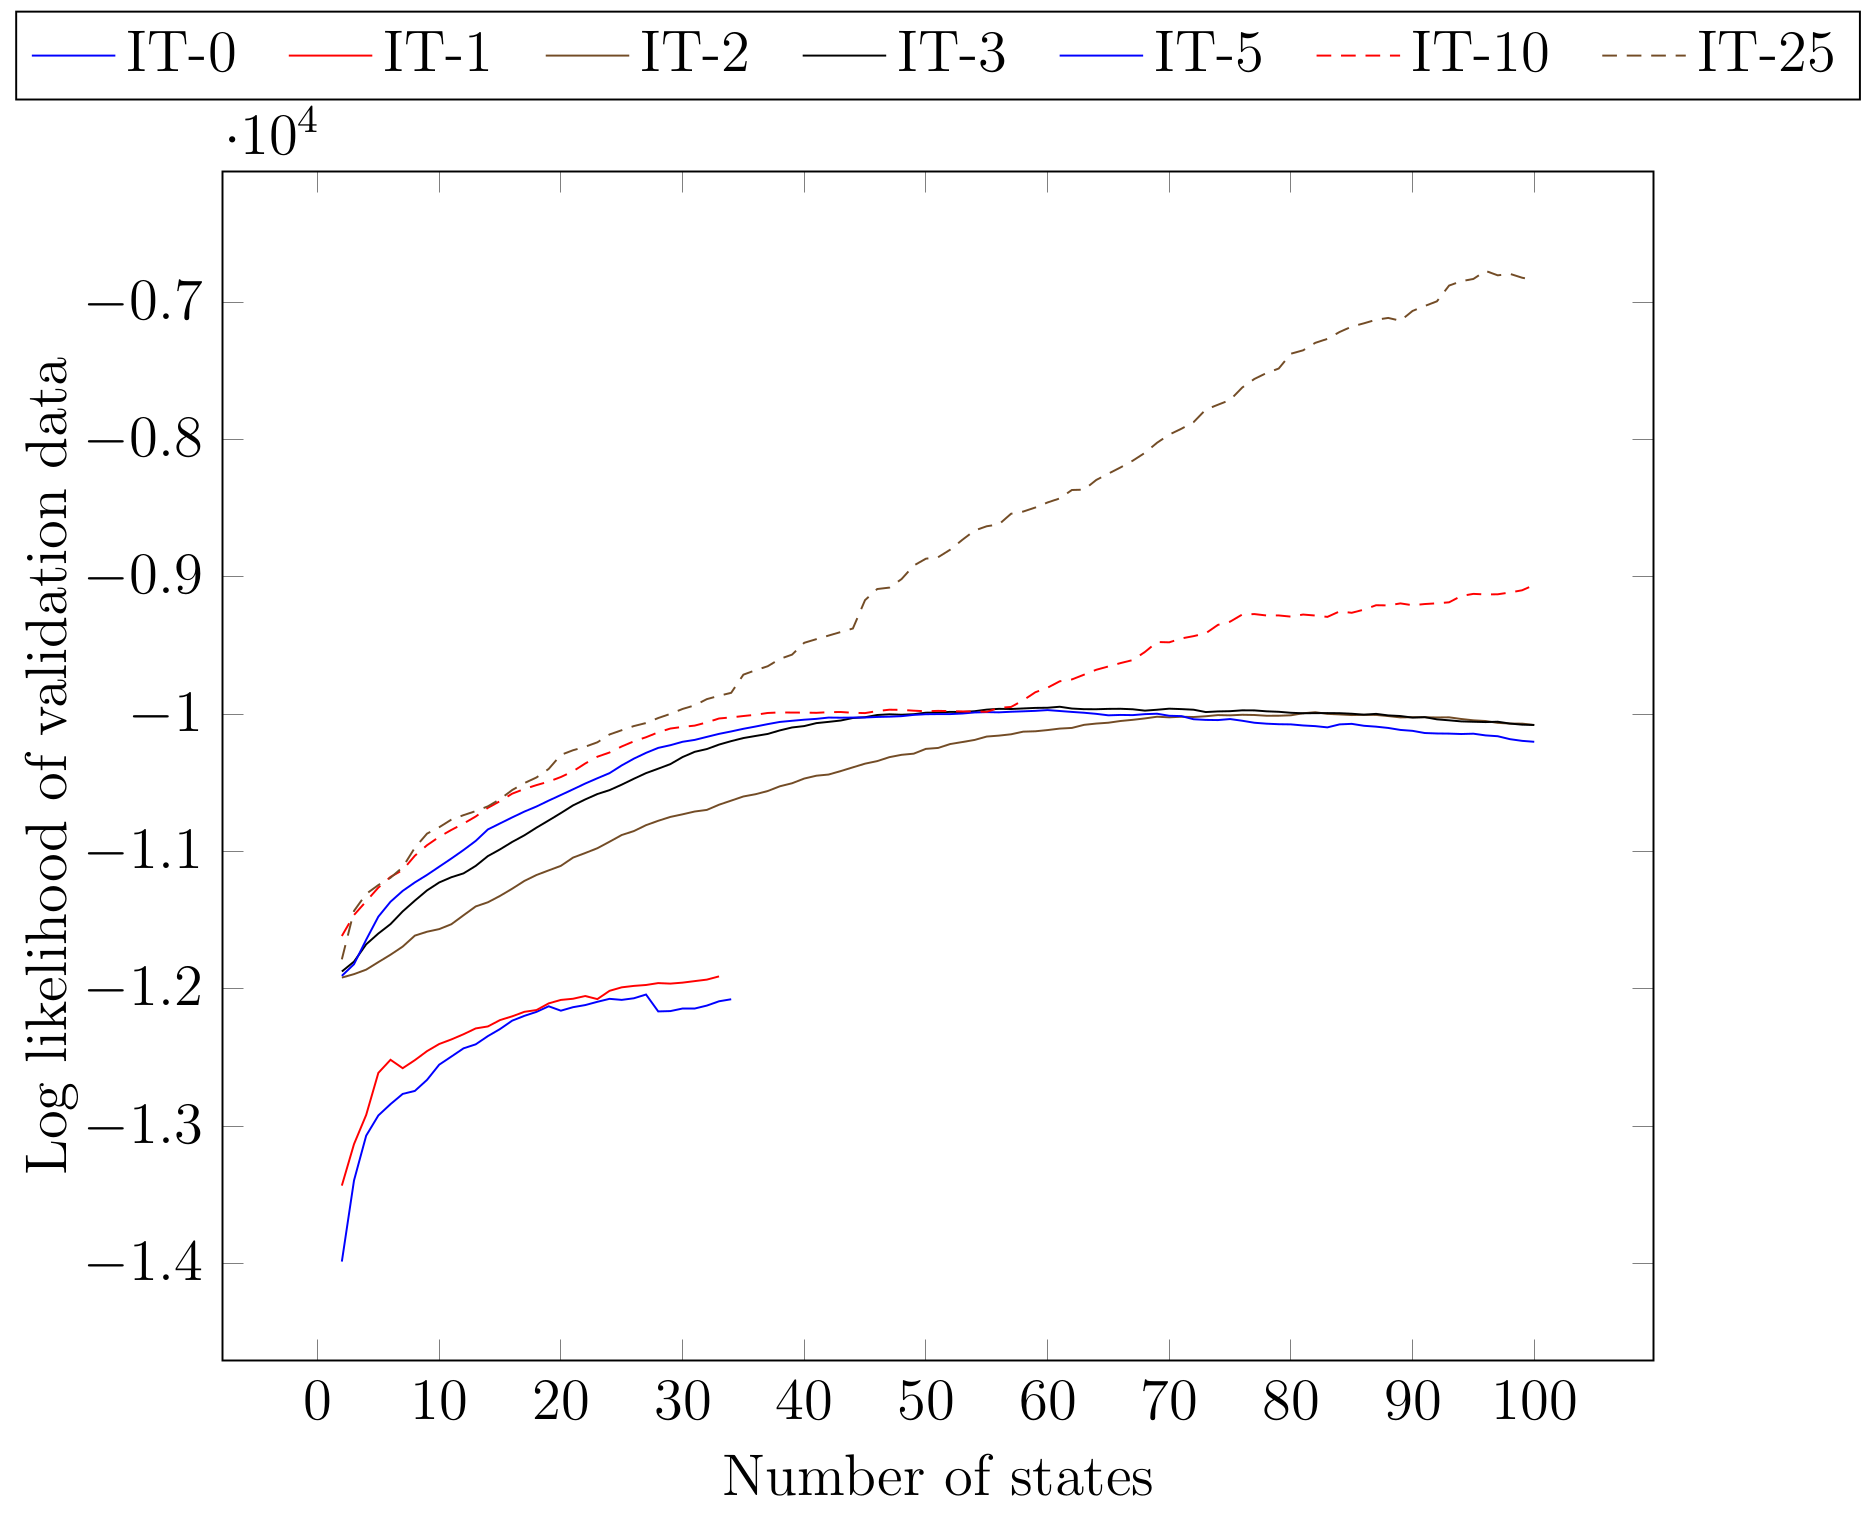
\includegraphics[width=0.9\textwidth]{images/beta.png}
	\end{centering}
\end{frame}

\section{\scshape Experiments}
\subsection{this shit}

\begin{frame}
\center \huge \scshape Experiments
\end{frame}

\begin{frame}
  \frametitle{Experiments}
  \begin{itemize}
  	\item Training - 5000 sequences
  	\item Validation - 5000 sequences
  	\item States - 10 to 100
  	\item How does problem characteristics affect prediction accuracy
  	\item Running time comparison
  \end{itemize}
\end{frame}

\begin{frame}
  \frametitle{State space}
\begin{figure}
\centering
\textbf{Data set: 6, States: 19}\par\medskip
\begin{tikzpicture}[scale=0.8]
	\pgfplotsset{every axis legend/.append style={ 
		at={(0.5,1.1)},
		anchor=south}}
	\begin{axis}[
			scaled ticks = true,
			scaled y ticks=base 10:-4,
			xlabel = Number of states,
            	ylabel = Log likelihood,
            	legend columns=-1,
            	legend entries={BW, SBW, GE, GS},
			legend style={/tikz/every even column/.append style={column sep=0.3cm}}]
			
		\addplot+table[x=States, y=BW, col sep=tab]
		{graphdata/set6.csv};
%		\addlegendentry{\textbf{BW}}
		
		\addplot+table[x=States, y=SBW, col sep=tab]
		{graphdata/set6.csv};
%		\addlegendentry{\textbf{Sparse BW}}
		
		\addplot+table[x=States, y=GE, col sep=tab]
		{graphdata/set6.csv};
		
		\addplot+table[x=States, y=Padawan, col sep=tab]
		{graphdata/set6.csv};
%		\addlegendentry{\textbf{Greedy Extend}}
	\end{axis}
\end{tikzpicture} 
\end{figure}
\end{frame}

\begin{frame}
  \frametitle{State space}
\begin{figure}
\centering
\textbf{Data set: 23, States: 33}\par\medskip
\begin{tikzpicture}[scale=0.8]
	\pgfplotsset{every axis legend/.append style={ 
		at={(0.5,1.1)},
		anchor=south}}
	\begin{axis}[
			scaled ticks = true,
			scaled y ticks=base 10:-4,
			xlabel = Number of states,
            	ylabel = Log likelihood,
            	legend columns=-1,
            	legend entries={BW, SBW, GE, GS},
			legend style={/tikz/every even column/.append style={column sep=0.3cm}}]
			
		\addplot+table[x=States, y=BW, col sep=tab]
		{graphdata/set23.csv};
%		\addlegendentry{\textbf{BW}}
		
		\addplot+table[x=States, y=SBW, col sep=tab]
		{graphdata/set23.csv};
%		\addlegendentry{\textbf{Sparse BW}}
		
		\addplot+table[x=States, y=GE, col sep=tab]
		{graphdata/set23.csv};
		
		\addplot+table[x=States, y=Padawan, col sep=tab]
		{graphdata/set23.csv};
%		\addlegendentry{\textbf{Greedy Extend}}
	\end{axis}
\end{tikzpicture}
\end{figure}
\end{frame}

 
\begin{frame}
  \frametitle{State space}
\begin{figure}
\centering
\textbf{Data set: 41, States: 54}\par\medskip
\begin{tikzpicture}[scale=0.8]
	\pgfplotsset{every axis legend/.append style={ 
		at={(0.5,1.1)},
		anchor=south}}
	\begin{axis}[
			scaled ticks = true,
			scaled y ticks=base 10:-4,
			xlabel = Number of states,
            	ylabel = Log likelihood,
            	legend columns=-1,
            	legend entries={BW, SBW, GE, GS},
			legend style={/tikz/every even column/.append style={column sep=0.3cm}}]
			
		\addplot+table[x=States, y=BW, col sep=tab]
		{graphdata/set41.csv};
%		\addlegendentry{\textbf{BW}}
		
		\addplot+table[x=States, y=SBW, col sep=tab]
		{graphdata/set41.csv};
%		\addlegendentry{\textbf{Sparse BW}}
		
		\addplot+table[x=States, y=GE, col sep=tab]
		{graphdata/set41.csv};
		
		\addplot+table[x=States, y=Padawan, col sep=tab]
		{graphdata/set41.csv};
%		\addlegendentry{\textbf{Greedy Extend}}
	\end{axis}
\end{tikzpicture} 
\end{figure}
\end{frame}

\begin{frame}
  \frametitle{State space}
\begin{figure}
\centering
\textbf{Data set: 1, States: 64}\par\medskip
\begin{tikzpicture}[scale=0.8]
	\pgfplotsset{every axis legend/.append style={ 
		at={(0.5,1.1)},
		anchor=south}}
	\begin{axis}[
			scaled ticks = true,
			scaled y ticks=base 10:-4,
			xlabel = Number of states,
            	ylabel = Log likelihood,
            	legend columns=-1,
            	legend entries={BW, SBW, GE, GS},
			legend style={/tikz/every even column/.append style={column sep=0.3cm}}]
			
		\addplot+table[x=States, y=BW, col sep=tab]
		{graphdata/set1.csv};
%		\addlegendentry{\textbf{BW}}
		
		\addplot+table[x=States, y=SBW, col sep=tab]
		{graphdata/set1.csv};
%		\addlegendentry{\textbf{Sparse BW}}
		
		\addplot+table[x=States, y=GE, col sep=tab]
		{graphdata/set1.csv};
		
		\addplot+table[x=States, y=Padawan, col sep=tab]
		{graphdata/set1.csv};
%		\addlegendentry{\textbf{Greedy Extend}}
	\end{axis}
\end{tikzpicture} 
\end{figure}
\end{frame}

\begin{frame}
  \frametitle{Transition sparsity}
\begin{figure} 
	\centering
	\textbf{Dataset: 36, Sparsity: 7.4\%}\par\medskip
  	\begin{tikzpicture}[scale=0.8]
	\pgfplotsset{every axis legend/.append style={ 
		at={(0.5,1.1)},
		anchor=south}}
	\begin{axis}[
			scaled ticks = true,
			scaled y ticks=base 10:-4,
			xlabel = Number of states,
            	ylabel = Log likelihood,
            	legend columns=-1,
            	legend entries={BW, SBW, GE, GS},
			legend style={/tikz/every even column/.append style={column sep=0.3cm}}]
		
		\addplot+table[x=States, y=BW, col sep=tab]
		{graphdata/set36.csv};
%		\addlegendentry{\textbf{BW}}
		
		\addplot+table[x=States, y=SBW, col sep=tab]
		{graphdata/set36.csv};
%		\addlegendentry{\textbf{Sparse BW}}
		
		\addplot+table[x=States, y=GE, col sep=tab]
		{graphdata/set36.csv};
		
		\addplot+table[x=States, y=Padawan, col sep=tab]
		{graphdata/set36.csv};
%		\addlegendentry{\textbf{Greedy Extend}}
	\end{axis}
	
\end{tikzpicture} 
\end{figure} 
\end{frame}

\begin{frame}
 \frametitle{Transition sparsity}
\begin{figure}
\centering
\textbf{Dataset: 8, Sparsity: 16.8\%}\par\medskip
\begin{tikzpicture}[scale=0.8]
	\pgfplotsset{every axis legend/.append style={ 
		at={(0.5,1.1)},
		anchor=south}}
	\begin{axis}[
			scaled ticks = true,
			scaled y ticks=base 10:-4,
			xlabel = Number of states,
            	ylabel = Log likelihood,
            	legend columns=-1,
            	legend entries={BW, SBW, GE, GS},
			legend style={/tikz/every even column/.append style={column sep=0.3cm}}]
		
		\addplot+table[x=States, y=BW, col sep=tab]
		{graphdata/set8.csv};
%		\addlegendentry{\textbf{BW}}
		
		\addplot+table[x=States, y=SBW, col sep=tab]
		{graphdata/set8.csv};
%		\addlegendentry{\textbf{Sparse BW}}
		
		\addplot+table[x=States, y=GE, col sep=tab]
		{graphdata/set8.csv};
	
		\addplot+table[x=States, y=Padawan, col sep=tab]
		{graphdata/set8.csv};
%		\addlegendentry{\textbf{Greedy Extend}}
	\end{axis}
\end{tikzpicture}
\end{figure}
\end{frame}

\begin{frame}
 \frametitle{Transition sparsity}
\begin{figure}
\centering
\textbf{Dataset: 43, Sparsity: 40.2\%}\par\medskip
\begin{tikzpicture}[scale=0.8]
	\pgfplotsset{every axis legend/.append style={ 
		at={(0.5,1.1)},
		anchor=south}}
	\begin{axis}[
			scaled ticks = true,
			scaled y ticks=base 10:-4,
			xlabel = Number of states,
            	ylabel = Log likelihood,
            	legend columns=-1,
            	legend entries={BW, SBW, GE, GS},
			legend style={/tikz/every even column/.append style={column sep=0.3cm}}]
			
		\addplot+table[x=States, y=BW, col sep=tab]
		{graphdata/set43.csv};
%		\addlegendentry{\textbf{BW}}
		
		\addplot+table[x=States, y=SBW, col sep=tab]
		{graphdata/set43.csv};
%		\addlegendentry{\textbf{Sparse BW}}
		
		\addplot+table[x=States, y=GE, col sep=tab]
		{graphdata/set43.csv};
		
		\addplot+table[x=States, y=Padawan, col sep=tab]
		{graphdata/set43.csv};
%		\addlegendentry{\textbf{Greedy Extend}}
	\end{axis}
\end{tikzpicture} 
\end{figure}
\end{frame}

\begin{frame}
 \frametitle{Transition sparsity}
\begin{figure}
\centering
\textbf{Dataset: 37, Sparsity: 50\%}\par\medskip
\begin{tikzpicture}[scale=0.8]
	\pgfplotsset{every axis legend/.append style={ 
		at={(0.5,1.1)},
		anchor=south}}
	\begin{axis}[
			scaled ticks = true,
			scaled y ticks=base 10:-4,
			xlabel = Number of states,
            	ylabel = Log likelihood,
            	legend columns=-1,
            	legend entries={BW, SBW, GE, GS},
			legend style={/tikz/every even column/.append style={column sep=0.3cm}}]
			
		\addplot+table[x=States, y=BW, col sep=tab]
		{graphdata/set37.csv};
%		\addlegendentry{\textbf{BW}}
		
		\addplot+table[x=States, y=SBW, col sep=tab]
		{graphdata/set37.csv};
%		\addlegendentry{\textbf{Sparse BW}}
		
		\addplot+table[x=States, y=GE, col sep=tab]
		{graphdata/set37.csv};
		
		\addplot+table[x=States, y=Padawan, col sep=tab]
		{graphdata/set37.csv};
%		\addlegendentry{\textbf{Greedy Extend}}
	\end{axis}
\end{tikzpicture} 
\end{figure}
\end{frame}


\begin{frame}
  \frametitle{Alphabet size}
\begin{figure}
\centering
\textbf{Dataset: 32, Symbols: 4}\par\medskip
\begin{tikzpicture}[scale=0.8]
	\pgfplotsset{every axis legend/.append style={ 
		at={(0.5,1.1)},
		anchor=south}}
	\begin{axis}[
			scaled ticks = true,
			scaled y ticks=base 10:-4,
			xlabel = Number of states,
            	ylabel = Log likelihood,
            	legend columns=-1,
            	legend entries={BW, SBW, GE, GS},
			legend style={/tikz/every even column/.append style={column sep=0.3cm}}]
			
		\addplot+table[x=States, y=BW, col sep=tab]
		{graphdata/set32.csv};
%		\addlegendentry{\textbf{BW}}
		
		\addplot+table[x=States, y=SBW, col sep=tab]
		{graphdata/set32.csv};
%		\addlegendentry{\textbf{Sparse BW}}
		
		\addplot+table[x=States, y=GE, col sep=tab]
		{graphdata/set32.csv};
		
		\addplot+table[x=States, y=Padawan, col sep=tab]
		{graphdata/set32.csv};
%		\addlegendentry{\textbf{Greedy Extend}}
	\end{axis}
\end{tikzpicture} 
\end{figure}
\end{frame}

\begin{frame}
  \frametitle{Alphabet size}
\begin{figure}
\centering
\textbf{Dataset: 8, Symbols: 8}\par\medskip
\begin{tikzpicture}[scale=0.8]
	\pgfplotsset{every axis legend/.append style={ 
		at={(0.5,1.1)},
		anchor=south}}
	\begin{axis}[
			scaled ticks = true,
			scaled y ticks=base 10:-4,
			xlabel = Number of states,
            	ylabel = Log likelihood,
            	legend columns=-1,
            	legend entries={BW, SBW, GE, GS},
			legend style={/tikz/every even column/.append style={column sep=0.3cm}}]
			
		\addplot+table[x=States, y=BW, col sep=tab]
		{graphdata/set8.csv};
%		\addlegendentry{\textbf{BW}}
		
		\addplot+table[x=States, y=SBW, col sep=tab]
		{graphdata/set8.csv};
%		\addlegendentry{\textbf{Sparse BW}}
		
		\addplot+table[x=States, y=GE, col sep=tab]
		{graphdata/set8.csv};
		
		\addplot+table[x=States, y=Padawan, col sep=tab]
		{graphdata/set8.csv};
%		\addlegendentry{\textbf{Greedy Extend}}
	\end{axis}
\end{tikzpicture} 
\end{figure}
\end{frame}

\begin{frame}
  \frametitle{Alphabet size}
\begin{figure}
\centering
\textbf{Dataset: 10, Symbols: 11}\par\medskip
\begin{tikzpicture}[scale=0.8]
	\pgfplotsset{every axis legend/.append style={ 
		at={(0.5,1.1)},
		anchor=south}}
	\begin{axis}[
			scaled ticks = true,
			scaled y ticks=base 10:-4,
			xlabel = Number of states,
            	ylabel = Log likelihood,
            	legend columns=-1,
            	legend entries={BW, SBW, GE, GS},
			legend style={/tikz/every even column/.append style={column sep=0.3cm}}]
			
		\addplot+table[x=States, y=BW, col sep=tab]
		{graphdata/set10.csv};
%		\addlegendentry{\textbf{BW}}
		
		\addplot+table[x=States, y=SBW, col sep=tab]
		{graphdata/set10.csv};
%		\addlegendentry{\textbf{Sparse BW}}
		
		\addplot+table[x=States, y=GE, col sep=tab]
		{graphdata/set10.csv};
		
		\addplot+table[x=States, y=Padawan, col sep=tab]
		{graphdata/set10.csv};
%		\addlegendentry{\textbf{Greedy Extend}}
	\end{axis}
\end{tikzpicture}
\end{figure}
\end{frame}

\begin{frame}
  \frametitle{Alphabet size}
\begin{figure}
\centering
\textbf{Dataset: 35, Symbols: 20}\par\medskip
\begin{tikzpicture}[scale=0.8]
	\pgfplotsset{every axis legend/.append style={ 
		at={(0.5,1.1)},
		anchor=south}}
	\begin{axis}[
			scaled ticks = true,
			scaled y ticks=base 10:-4,
			xlabel = Number of states,
            	ylabel = Log likelihood,
            	legend columns=-1,
            	legend entries={BW, SBW, GE, GS},
			legend style={/tikz/every even column/.append style={column sep=0.3cm}}]
			
		\addplot+table[x=States, y=BW, col sep=tab]
		{graphdata/set35.csv};
%		\addlegendentry{\textbf{BW}}
		
		\addplot+table[x=States, y=SBW, col sep=tab]
		{graphdata/set35.csv};
%		\addlegendentry{\textbf{Sparse BW}}
		
		\addplot+table[x=States, y=GE, col sep=tab]
		{graphdata/set35.csv};
		
		\addplot+table[x=States, y=Padawan, col sep=tab]
		{graphdata/set35.csv};
%		\addlegendentry{\textbf{Greedy Extend}}
	\end{axis}
\end{tikzpicture}
\end{figure}
\end{frame}

\begin{frame}
  \frametitle{Speed comparison}
\begin{figure}
\begin{figure}
	\centering
	\begin{tikzpicture}[scale=0.9]
		\begin{axis}[
			width=0.92\textwidth,
			height=0.76\textheight,
		%	ymax=0,
		%	xmax=0,
			xlabel = Number of states,
            		ylabel = Log likelihood,
            		legend style={at={(0,1)}, anchor=north west}]
			\addplot+[mark=none]table[x=States, y=Score, col sep=tab]
			{graphdata/8h_run_BW.csv};
			\addlegendentry{Baum-Welch Learner}
			\addplot+[mark=none]table[x=States, y=Score, col sep=tab]
			{graphdata/8h_run_SBW.csv};
			\addlegendentry{Sparse Baum-Welch Learner}
			\addplot+[mark=none]table[x=States, y=Score, col sep=tab]
			{graphdata/8h_run_GE.csv};
			\addlegendentry{Greedy Extend Learner}
		\end{axis}
	\end{tikzpicture}
	\caption{Results achieved in a time scope of eight hours.}
\end{figure}
\end{figure}
\end{frame}

\begin{frame}
  \frametitle{Speed comparison}
\begin{figure}
	\centering
	\begin{tikzpicture}[scale=0.9]
		\begin{axis}[
			ymin=0,
			xmin=0,
			xlabel = Number of states,
            		ylabel = Time until convergence {[s]},
            		legend style={at={(0,1)}, anchor=north west}]
			\addplot+table[x=States, y=Time, col sep=tab]
			{graphdata/8h_run_BW.csv};
			\addlegendentry{Baum-Welch Learner}
			\addplot+table[x=States, y=Time, col sep=tab]
			{graphdata/8h_run_SBW.csv};
			\addlegendentry{Sparse Baum-Welch Learner}
		\end{axis}
	\end{tikzpicture}
	\caption{Running time comparison between Baum-Welch and Sparse Baum-Welch Learners}
	\label{fig:bw_vs_sbw}
\end{figure}
\end{frame}

\section{\scshape Experiments}
\subsection{Results}

\begin{frame}
  \frametitle{Results}
  \begin{itemize}
  	\item 3 data sets: 6, 23, 35
  	\item Parameters chosen based on the experiments presented earlier
  	\item 5000 sequences
  	\item Static: 10 initial states, step size 10
  	\item Dynamic: 10 initial states, 5 intermediate BW iterations
  \end{itemize}
\end{frame}

\begin{frame}
  \frametitle{Results} 
  \begin{center}
	\begin{table}[h]
		\centering
		\begin{tabular}{|c|r|r|r|r|r|}
		\hline
		Data set    & \multicolumn{1}{c|}{\textbf{GE}} & \multicolumn{1}{c|}{\textbf{BW}} & \multicolumn{1}{c|}{\textbf{SBW}} & \multicolumn{1}{c|}{\textbf{GS}} & \multicolumn{1}{c|}{\textbf{Goal}} \\ \hline
\textbf{6}  & 115.53                           & 122.60                           & 129.64                            & 114.77                           & 66.98                              		\\ \hline
		\textbf{23} & 26.30                            & 26.16                            & 26.08                             & 26.19                            & 18.41                              		\\ \hline
		\textbf{35} & 49.48                            & 43.36                            & 50.79                             & 44.44                            & 33.78                              		\\ \hline
		\end{tabular}
	\caption{The best scores of each algorithm on the three data sets.}
	\label{table:pautomac-best-score}
	\end{table}
  \end{center}
\end{frame}
	
\begin{frame}
  \frametitle{Results} 
  \begin{center}
	\begin{figure}
\centering
\begin{tikzpicture}[scale=0.80]
	\pgfplotsset{every axis legend/.append style={ 
		at={(0.5,1.1)},
		anchor=south}}
	\begin{axis}[
			xmin = 0,
			xmax = 100,
			ymin = 18,
			ymax = 38,
			cycle list name=color list,
			xlabel = States,
            	ylabel = Perplexity (lower is better),
            	legend columns=-1,
            	legend entries={GE, BW, SBW, GS, Goal},
			legend style={/tikz/every even column/.append style={column sep=0.3cm}},
			cycle list name=exotic]
		
		\addplot+[mark=none]table[x=States, y=GE, col sep=tab]
		{graphdata/pautomac-competition-results-dataset-23.csv};
		
		\addplot+[mark=none]table[x=States, y=BW, col sep=tab]
		{graphdata/pautomac-competition-results-dataset-23.csv};
		
		\addplot+[mark=none]table[x=States, y=SBW, col sep=tab]
		{graphdata/pautomac-competition-results-dataset-23.csv};
		
		\addplot+[mark=none]table[x=States, y=GS, col sep=tab]
		{graphdata/pautomac-competition-results-dataset-23.csv};
		
		\addplot+[mark=none]table[x=States, y=Goal, col sep=tab]
		{graphdata/pautomac-competition-results-dataset-23.csv};
	\end{axis}
\end{tikzpicture}
\caption{The different algorithm's score on \emph{PAutomaC}'s 23rd data set, according to the perplexity measure used in the competition.}
\label{fig:pautomac-competition-23}
\end{figure}
  \end{center}
\end{frame}


\section{\scshape Conclusion}
\subsection{Conclusion}
\begin{frame}
\center \huge \scshape Conclusion
\end{frame}

\begin{frame}
  \frametitle{Conclusion}
  \begin{itemize}
  	\item Analysis of different approaches using a sparse transition matrix in the BW algorithm
  	\item Dynamic algorithms: about as good results as BW when not better
  	\item Sparse matrix ensured by adding states iteratively
  \end{itemize}
\end{frame}

\begin{frame}
  \frametitle{Conclusion: Pros and Cons}
  \begin{center}
	\begin{table}[h]
  \resizebox{\textwidth}{!}{ 
\begin{tabular}{|l|l|l|}
\hline
Algorithm & Advantages                                                                                & Drawbacks                                                                                 \\ \hline
GE        & \begin{tabular}[c]{@{}l@{}}- Rather fast\\ - Good results\end{tabular}                    & \begin{tabular}[c]{@{}l@{}}- Usually needs more states to \\   start to compare\end{tabular} \\ \hline
GS        & \begin{tabular}[c]{@{}l@{}}- Splitting heuristic\\ - Best results, but...\end{tabular}    & \begin{tabular}[c]{@{}l@{}}- Runs on a dense matrix\\ - ...unusual behaviour\end{tabular} \\ \hline
SBW       & \begin{tabular}[c]{@{}l@{}}- Computational speed-up\\ - Room for improvement\end{tabular} & \begin{tabular}[c]{@{}l@{}}- Results slightly worse than BW\\ - No speed-up on some data sets\end{tabular} \\ \hline
\end{tabular}
}
\end{table}
  \end{center}
\end{frame}

\begin{frame}
  \frametitle{Conclusion: Experiments conducted}
  \begin{itemize}
  	\item 3 types of experiment
  	\item 4 algorithms
  \end{itemize}
\end{frame}

\begin{frame}
  \frametitle{Conclusion: First experiments}
  \begin{itemize}
  	\item Extremely varied behaviour on different data sets
  	\item Three available parameters for results analysis
  	\item Hypotheses, but no definite clear pattern
  	\item In general, results on par with BW (sometimes outperforming it)
  \end{itemize}
\end{frame}

\begin{frame}
  \frametitle{Conclusion: Second experiments}
  \begin{itemize}
  	\item Speed comparison between: BW, SBW, GE
  	\item 8-hour run
  	\item GE dominating both in speed and in score
  	\item SBW unstable: random matrix causing non-deterministic behaviour (suggests buiding a data-derived one instead)
  \end{itemize}
\end{frame}

\begin{frame}
  \frametitle{Conclusion: Third experiments}
  \begin{itemize}
  	\item Comparison using PAutomaC scores
  	\item Unsatisfactory results, but...
  	\item ...due to a different paradigm used: no stopping probabilities have been used
  \end{itemize}
\end{frame}

\subsection{Future Work}

\begin{frame}
  \frametitle{Conclusion: Future work}
  \begin{itemize}
  	\item Eliminating possible noise
  	\item Explain the multitude of behaviours, validating or disproving our hypotheses
  	\item Running on more states
  	\item Comparing with the PAutomaC scores, using the same paradigm
  	\item Optimising the sparse transition matrices used in the algorithms
  	\item Making sure underflow and overfitting are avoided
  	\item Looking more in-depth into the other methods we have put aside in this project
  \end{itemize}
\end{frame}

\end{document}
